\chapter{Análisis espectral numérico de los PDL}
\label{chap: resultados numericos analisis espectrales}

Establecida ya la teoría necesaria
para definir todos los elementos de los espectros
basados en la TDF y en espacios monofrecuenciales 
de una señal finita $x \in \IR^{n}$,
programando la funciones necesarias para realizar análisis espectrales
de los polinomios discretos de Legendre
usando estas dos metodologías; podremos así
comprobar o refutar y mejorar
la hipótesis hecha en 
\ref{ref: hipotesis}. 

Puede encontrar el código, implementado en Python,
en \TODO{cita al repositorio.} \\

Antes de mostrar las gráficas de los espectros
de algunos PDL, 
redactamos en la siguiente sección unas preguntas guía
que nos gustaría responder numéricamente, después de 
realizar análisis espectrales de los PDL
$\cali{L}^{n,k}$ de dimensión $2 \leq 2 \leq 69$. \\

No realizamos el análisis espectral para dimensiones
mayores a $69$ pues, para dimensiones más grandes, los números
involucrados en los cálculos son tan pequeños
en magnitud que son redondeados a cero
\sidenote{Puede consultar \cite{DSmath} para ver los detalles de cómo los
datos de tipo \texttt{float} son manipulados por la computadora
y los problemas de aproximación y redondeo que están implícitos en
este tipo de operaciones.}

\section{Preguntas a responder numéricamente sobre las oscilaciones de los PDL}

Enlistamos las preguntas que nos interesa considerar
relacionadas a las naturaleza oscilatoria
de los PDL $\cali{L}^{n,k}$
para dimensiones hasta $n=69$. 
Todas ellas se formulan con la intención de 
verificar o refutar y refinar la 
hipótesis \ref{ref: hipotesis} 
hecha al inicio del capítulo. La primera
de estas preguntas es una reformulación
de dicha hipótesis
en términos de los 
valores $FP0(x)$ y $FP1(x)$ definidos en 
\ref{def: FM0} y \ref{def: FM1}.

\begin{pregunta}
\label{pregunta 1}
Sean $2 \leq n \leq 69$ y $0 \leq k \leq n-1$.
Sea $\cali{L}^{n,k}$ el PDL de dimensión $n$ y grado $k$.
¿las frecuencias máximas
$FP0(\cali{L}^{n,k})$ y 
$FP1(\cali{L}^{n,k})$ son cercanas a $\frac{k}{2}$?
\end{pregunta}

A continuación mostramos un dibujo para
ilustrar cómo podrían verse los
espectros del PDL
$\cali{L}^{7,5} \in \IR^{7}$
en caso de que la respuesta a la pregunta
\ref{pregunta 1} sea afirmativa.
Observe que, en el segundo espectro,
fue posible usar varios valores de $\omega$ para analizar
a $\cali{L}^{7,5}$, y que podría ser que la frecuencia máxima
sea un número decimal, mientras que para el primer espectro
(el basado en la TDF) sólo pueden usarse algunas frecuencias
enteras, por lo que no esperamos que 
$FP0(x)$
sea $\frac{5}{2}$, pues este ni siquiera es un entero.
Esperamos, sin embargo, que el máximo se de en las frecuencias
enteras cercanas al valor $\frac{5}{2}$.

\begin{figure}[H]
	\sidecaption{
	A la izquierda un dibujo (no basado en datos reales) de 
	un posible espectro para $\cali{L}^{n,k}$ basado en la 
	DFT, y a la derecha uno basado en cosenos a espacios 
	monofrecuenciales. Observe que en el segundo espectro se pueden
	considerar muchas más frecuencias que en el primero.
	\label{fig: ejemplo_pregunta1}
	}
	\centering
	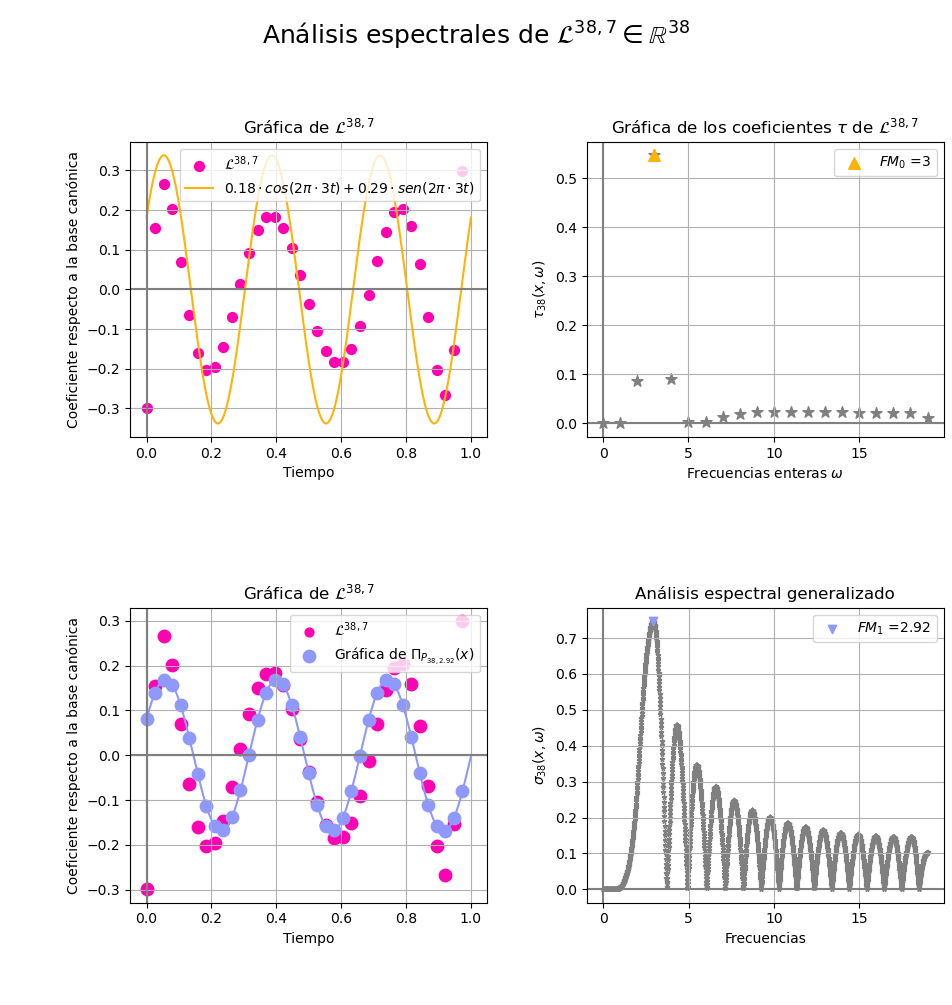
\includegraphics[scale = 0.9]{./estudios_espectrales/ejemplo_pregunta1} 
\end{figure}	

\begin{pregunta}
\label{preg 2}
¿Las frecuencias 
$FP0(\cali{L}^{n,k})$ y $FP1(\cali{L}^{n,k})$
dependen, como implica la pregunta 1, sólo del parámetro
de grado $k$ y no del de dimensión $n$?
Es decir, si $k$, $n_{1}$ y $n_{2}$
son tales que $k \leq n_{1}-1$ y
$k \leq n_{2}-1$, ¿ocurre que 
$FP0(\cali{L}^{n_{1},k})$ = $FP0(\cali{L}^{n_{2},k})$
y 
$FP1(\cali{L}^{n_{1},k})$ = $FP1(\cali{L}^{n_{2},k})$?
\end{pregunta}

Para tratar de responder a la pregunta \ref{preg 2},
fijado un grado $k$,
podría ser útil graficar los puntos de la forma
\begin{equation}
\label{eq0: 8may}
(n, FP0(\cali{L}^{n,k})), \hspace{0.2cm} k < n \leq 69,
\end{equation}
y 
\begin{equation}
\label{eq1: 8may}
(n, FP1(\cali{L}^{n,k})), \hspace{0.2cm} k < n \leq 69.
\end{equation}
Gráficas de este estilo podrían usarse para comprobar
la respuesta a la pregunta \ref{pregunta 1} 
graficando también la recta horizontal $y = \frac{k}{2}$
y viendo si los puntos graficados se encuentran cerca
de esta recta o no. 

\begin{figure}[H]
	\sidecaption{
	 De ser la respuesta
	a la pregunta \ref{preg 2} afirmativa, deberíamos
	de terminar con gráficas de puntos alineados horizontalmente, como
	en este dibujo. Sería bueno que los puntos $FP0$ y $FP1$ estuviesen
	a alturas parecidas, pues eso significaría que los dos análisis espectrales
	dan resultados parecidos.
	\label{fig: ejemplo_pregunta2}
	}
	\centering
	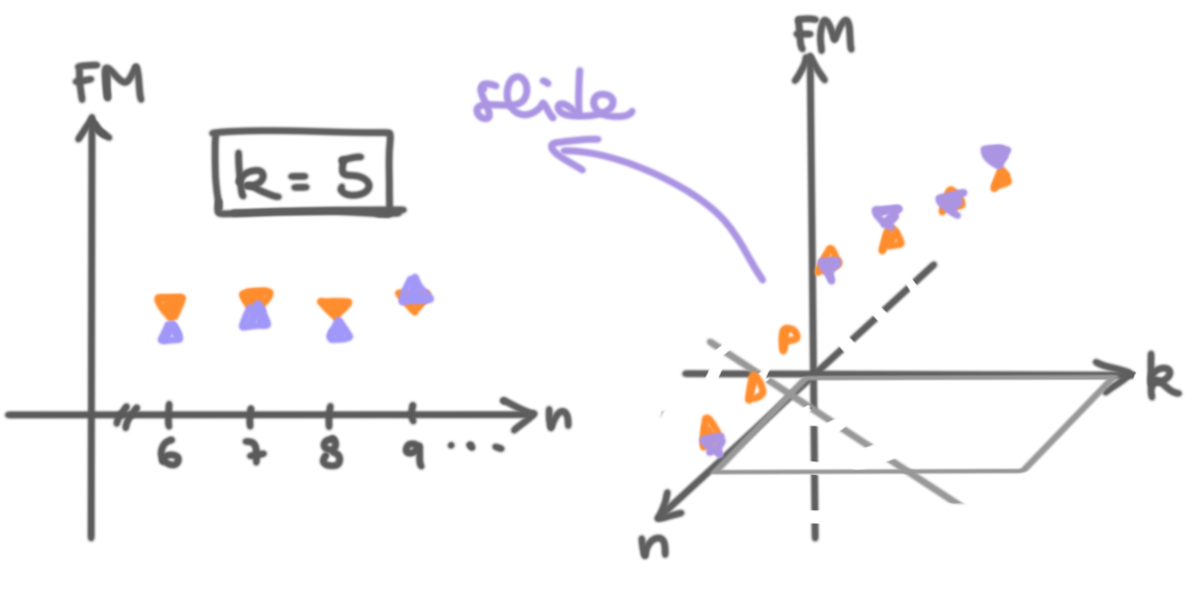
\includegraphics[scale = 1.4]{./estudios_espectrales/ejemplo_pregunta2} 
\end{figure}	


Para intentar refinar la aproximación hecha
en la hipótesis 
\ref{ref: hipotesis}, 
planteemos una tercera y última pregunta. 
Según esta hipótesis,
esperamos que tanto $FP0(\cali{L}^{n,k})$
como $FP1(\cali{L}^{n,k})$ sean cercanos a 
$\frac{k}{2}$; de ocurrir esto, tendríamos que los puntos de
las colecciones 
\begin{equation}
\label{eq5: May1}
(k, FP0(\cali{L}^{n,k})), \hspace{0.2cm} 0 \leq k \leq n-1
\end{equation}
y 
\begin{equation}
\label{eq6: May1}
(k, FP1(\cali{L}^{n,k})), \hspace{0.2cm} 0 \leq k \leq n-1,
\end{equation}
que se obtiene después de hacer análisis espectrales
a todos los PDL de dimensión $n$,
se ajustan a la recta $f(t) = \frac{t}{2}$. 
Una forma de comprobar o refutar esto es calcular las
rectas de mínimos cuadrados de estas dos colecciones
de puntos, y ver si las pendientes de estas son cercanas
a $1/2$ y las ordenadas al origen a $0$.
Planteamos esto en la siguiente


\begin{pregunta}
\label{preg 3}
Fijada una dimensión $2 \leq n \leq 69$,
considere las gráficas de los
puntos \eqref{eq5: May1}
y \eqref{eq6: May1}.

Sean $m_{n,0}$ y $b_{n,0}$ la pendiente y la ordenada
al origen de la recta de mínimos cuadrados calculada a 
partir del conjunto de puntos 
\eqref{eq5: May1}, y
$m_{n,1}$ y $b_{n,1}$ los correspondientes parámetros
para el conjunto de puntos 
\eqref{eq6: May1}.

Considere las nubes de puntos 
\[
(b_{n,0}, m_{n,0}), \hspace{0.2cm} 2 \leq n \leq 69
\]
y 
\[
(b_{n,1}, m_{n,1}), \hspace{0.2cm} 2 \leq n \leq 69.
\]
¿Alrededor de qué punto parecen concentrarse estas nubes?
\end{pregunta}

\begin{figure}[H]
	\sidecaption{
	Se muestran las gráficas 
	de las colecciones de puntos
	\eqref{eq5: May1} y \eqref{eq6: May1}
	para $n=7$	
	descritas en la pregunta
	\ref{preg 3}.
	\label{fig: ejemplo_pregunta3_0}
	}
	\centering
	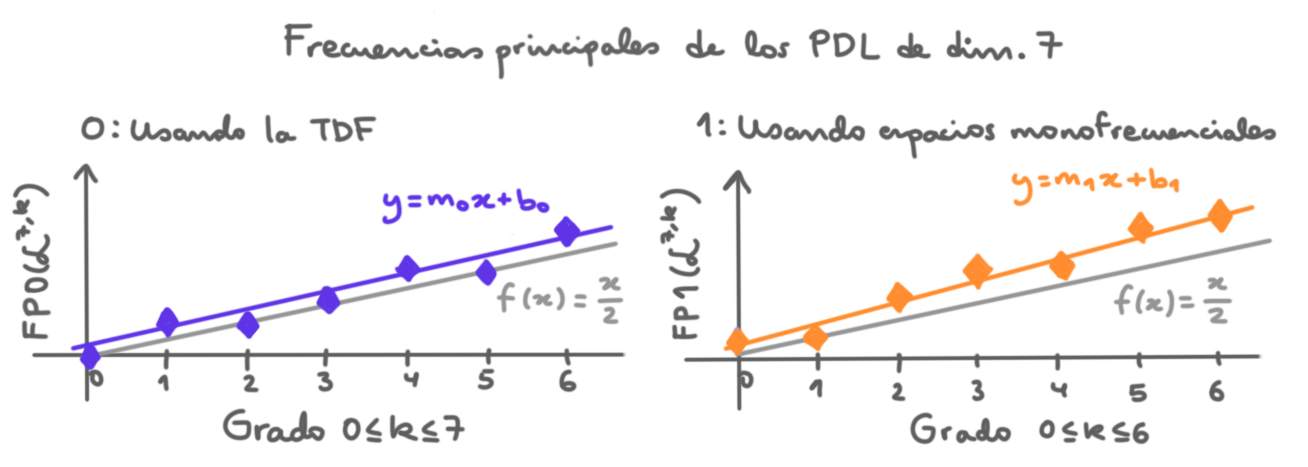
\includegraphics[scale = 1.1]{./estudios_espectrales/ejemplo_pregunta3_0} 
\end{figure}	

\begin{figure}[H]
	\sidecaption{
	Si la estimación dada en la pregunta \ref{pregunta 1} es
	buena, las nubes de puntos descritas en la 
	pregunta \ref{preg 3} deberían estar centradas
	en el punto $(0, 0.5)$.
	\label{fig: ejemplo_pregunta3_1}
	}
	\centering
	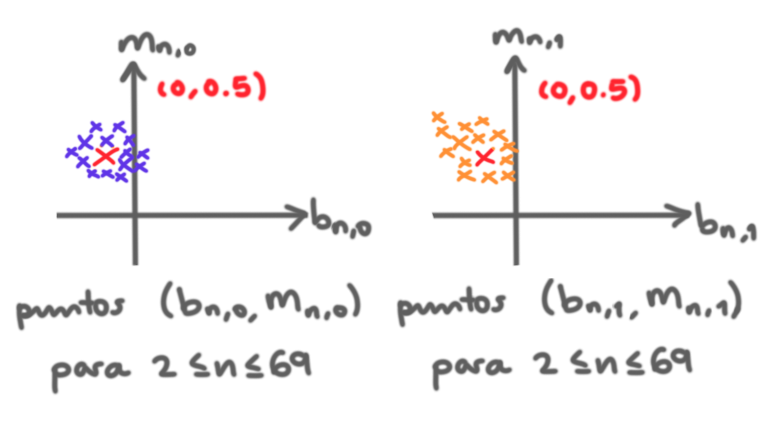
\includegraphics[scale = 1.5]{./estudios_espectrales/ejemplo_pregunta3} 
\end{figure}	


Vamos a responder a estas tres preguntas con gráficas parecidas
a las dibujadas en las figuras
\ref{fig: ejemplo_pregunta1},
\ref{fig: ejemplo_pregunta2},
\ref{fig: ejemplo_pregunta3_0} y
\ref{fig: ejemplo_pregunta3_1}. \\


Intentaremos responder a la pregunta \ref{pregunta 1}
con gráficas análogas
a las expuestas en el ejemplo
\ref{ej: espectros comparacion},
esta vez para analizar algunos PDL; la función con la que
hacemos esto es
\texttt{analisis$\_$espectrales$\_$PDL$\_$mostrarGrafica}. 
Para calcular los datos necesarios para responder
las preguntas \ref{preg 2} y \ref{preg 3},
usando la función \texttt{analisis$\_$espectralPDL$\_$global(n)}
(\TODO{referencia al código del repositorio}), 
para toda dimensión
$2 \leq n \leq 69$ calculamos
\begin{itemize}
	\item los coeficientes $FP1(\cali{L}^{n,k})$ para toda
	$0 \leq k \leq n-1$, y guardamos esta información en el
	array \texttt{sigmasMax$\_$n},
	\item los coeficientes $FP0(\cali{L}^{n,k})$ para toda
	$0 \leq k \leq n-1$, y guardamos esta información en el
	array \texttt{tausMax$\_$n},
	\item y los números $b_{n,0}$, $m_{n,0}$,
	$b_{n,1}$ y $m_{n,1}$ como se definieron en la pregunta
	\ref{preg 3}.
\end{itemize}
Toda esta información se calculó una sola vez y se almacenó
en un diccionario, cuyas llaves son las dimensiones
$n$, y cuyo valor asociado a la llave $n$ es la $6-$tupla
\[
(sigmasMax\_n, tausMax\_n, b_{n,0}, m_{n,0}, b_{n,1}, m_{n,1}).
\]

Usamos el 
módulo \texttt{pickle} para guardar los datos como secuencias
de bytes. El archivo binario en el que se almacenaron los
datos calculados con la función 
\texttt{analisis$\_$espectralPDL$\_$global(n)}
es \texttt{data$\_$AE.txt}. \\

La función con la que obtenemos gráficas análogas 
a la de la figura 
\ref{fig: ejemplo_pregunta2} es
\texttt{grafica$\_$analisisGlobal$\_$k$\_$fijo}
y, para obtener gráficas análogas a la de la figura
\ref{fig: ejemplo_pregunta3_0},
usamos \texttt{graficar$\_$analisis$\_$espectralPDL$\_$global}.

Recordamos que,
para cada análisis espectral,
vamos a tomar al conjunto de 
frecuencias 
como se sugiere en la nota \ref{nota: muestreo dom frecuencia}.

\section{Gráficas y comentarios}
Las gráficas de los espectros
para los PDL de dimensión hasta $40$, así
como gráficas análogas a las de las figuras
\ref{fig: ejemplo_pregunta2}
y 
\ref{fig: ejemplo_pregunta3_0}
se han guardado en \TODO{cita la carpeta del
repositorio
con las imágenes.}
A continuación, mostramos algunas
de estas imágenes con algunos comentarios
que nos ayuden a responder numéricamente a 
las preguntas
\ref{pregunta 1}, \ref{preg 2} y \ref{preg 3}
planteadas antes. \\

En todos los espectros que graficamos,
se resaltaron la recta horizontal
$y = 1$, para recordar que esa es la cota
superior de los coeficientes espectrales que
se grafican, 
y también la recta vertical $x = 0.5$. Según nuestra
hipótesis \ref{ref: hipotesis}, las frecuencias
principales debería estar cerca de esta recta vertical. \\

Veamos qué pasa con $n=7$.
Grafiquemos primero los espectros
de los PDL de dimensión $7$.

\begin{figure}[H]
	\sidecaption{
	\label{fig: 7_0}
	}
	\centering
	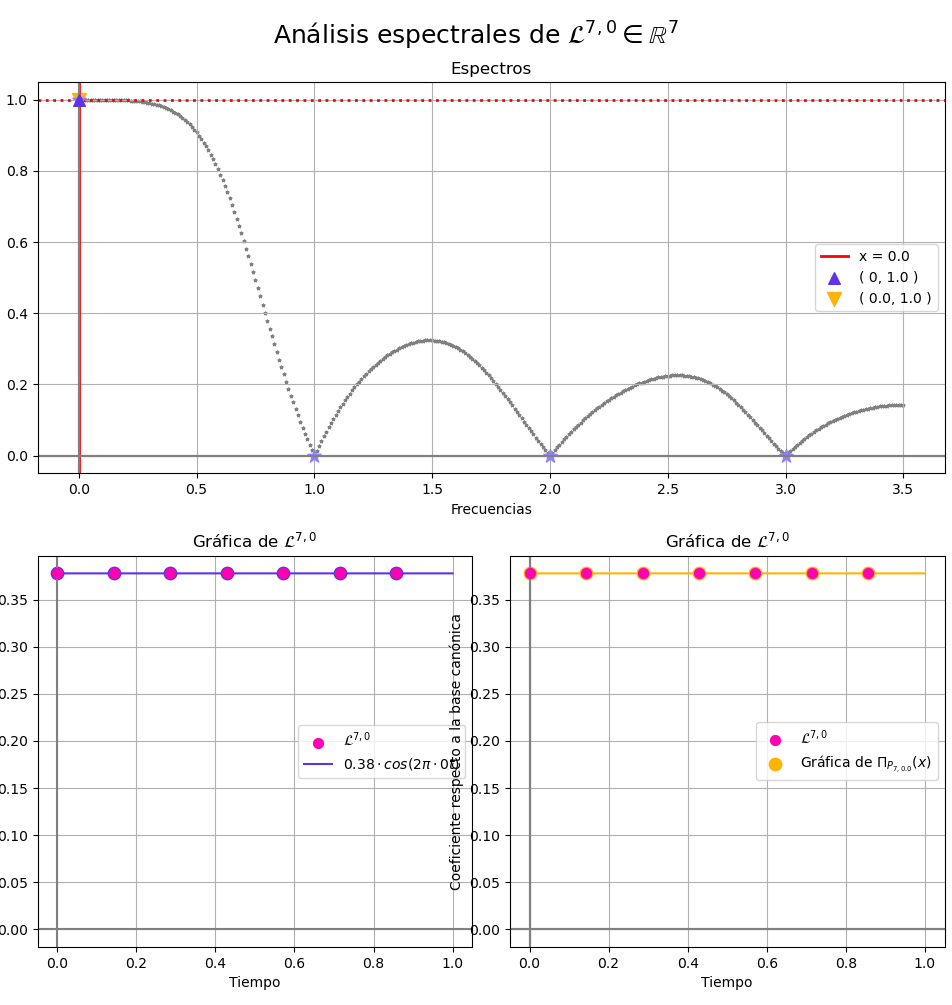
\includegraphics[scale = 0.3]{./graficas_analisisEspectrales/7_0} 
\end{figure}	

\begin{figure}[H]
	\sidecaption{
	\label{fig: 7_1}
	}
	\centering
	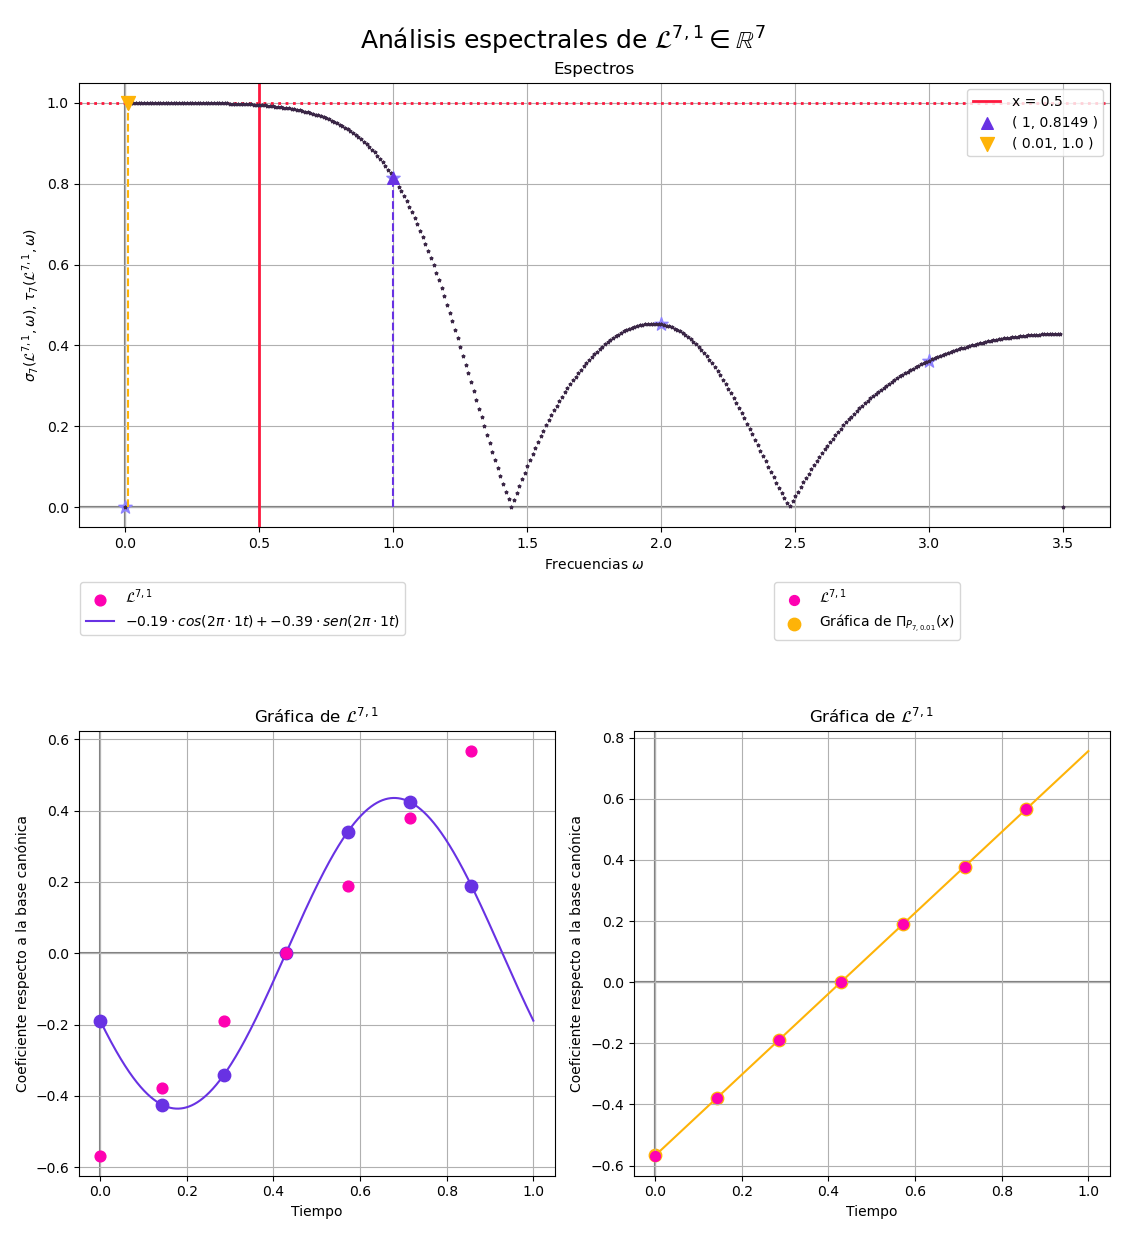
\includegraphics[scale = 0.3]{./graficas_analisisEspectrales/7_1} 
\end{figure}	

\begin{figure}[H]
	\sidecaption{
	\label{fig: 7_2}
	}
	\centering
	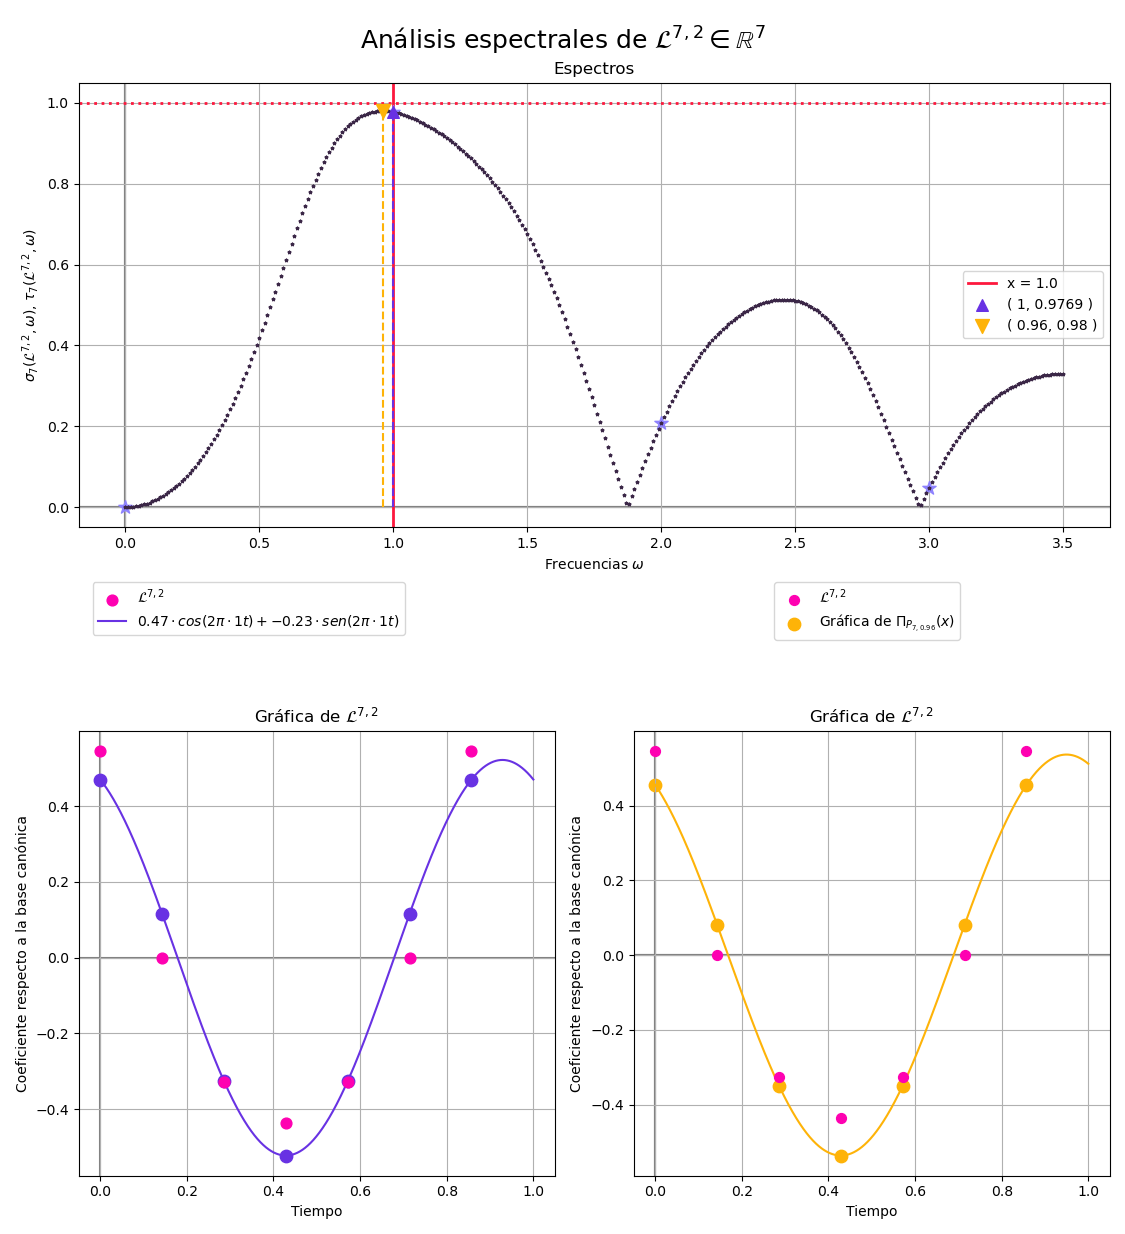
\includegraphics[scale = 0.3]{./graficas_analisisEspectrales/7_2} 
\end{figure}	


\begin{figure}[H]
	\sidecaption{
	\label{fig: 7_3}
	}
	\centering
	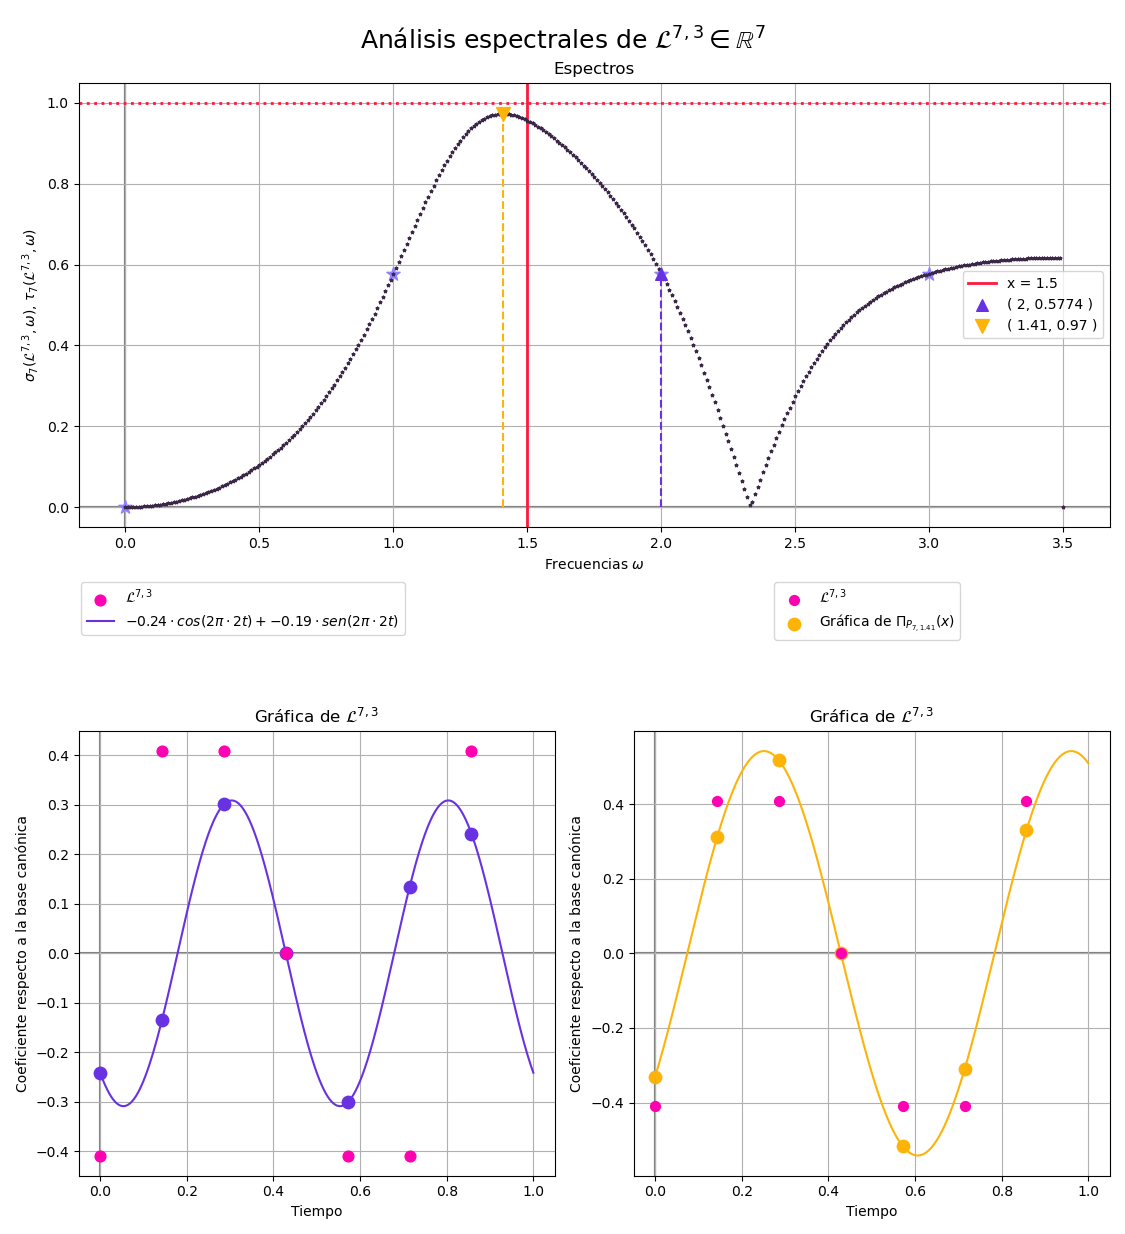
\includegraphics[scale = 0.3]{./graficas_analisisEspectrales/7_3} 
\end{figure}	


\begin{figure}[H]
	\sidecaption{
	\label{fig: 7_4}
	}
	\centering
	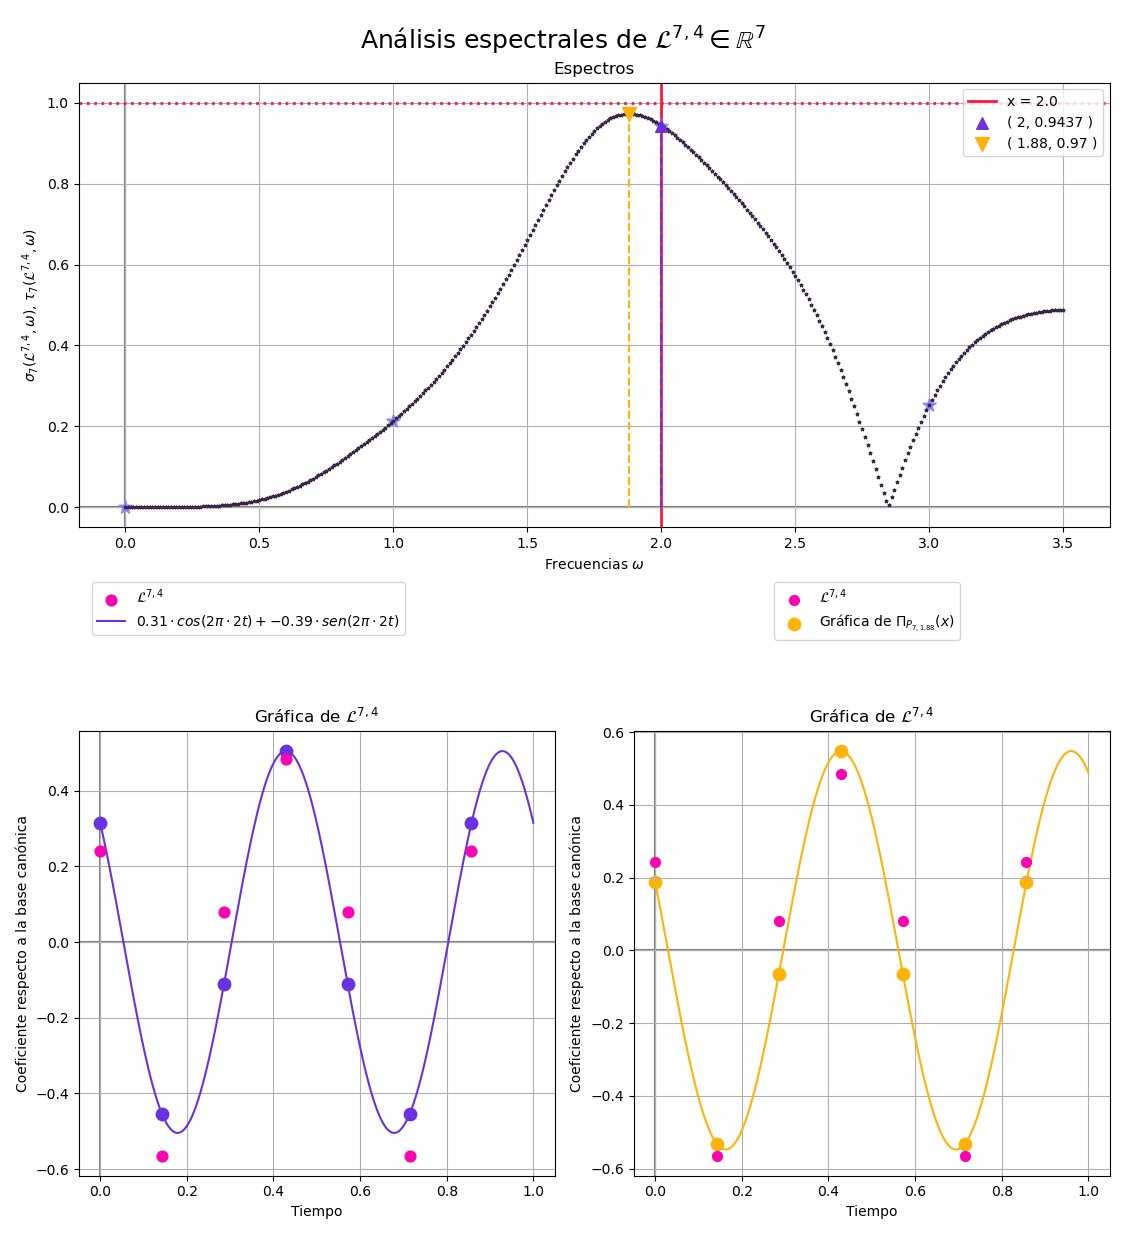
\includegraphics[scale = 0.3]{./graficas_analisisEspectrales/7_4} 
\end{figure}	


\begin{figure}[H]
	\sidecaption{
	\label{fig: 7_5}
	}
	\centering
	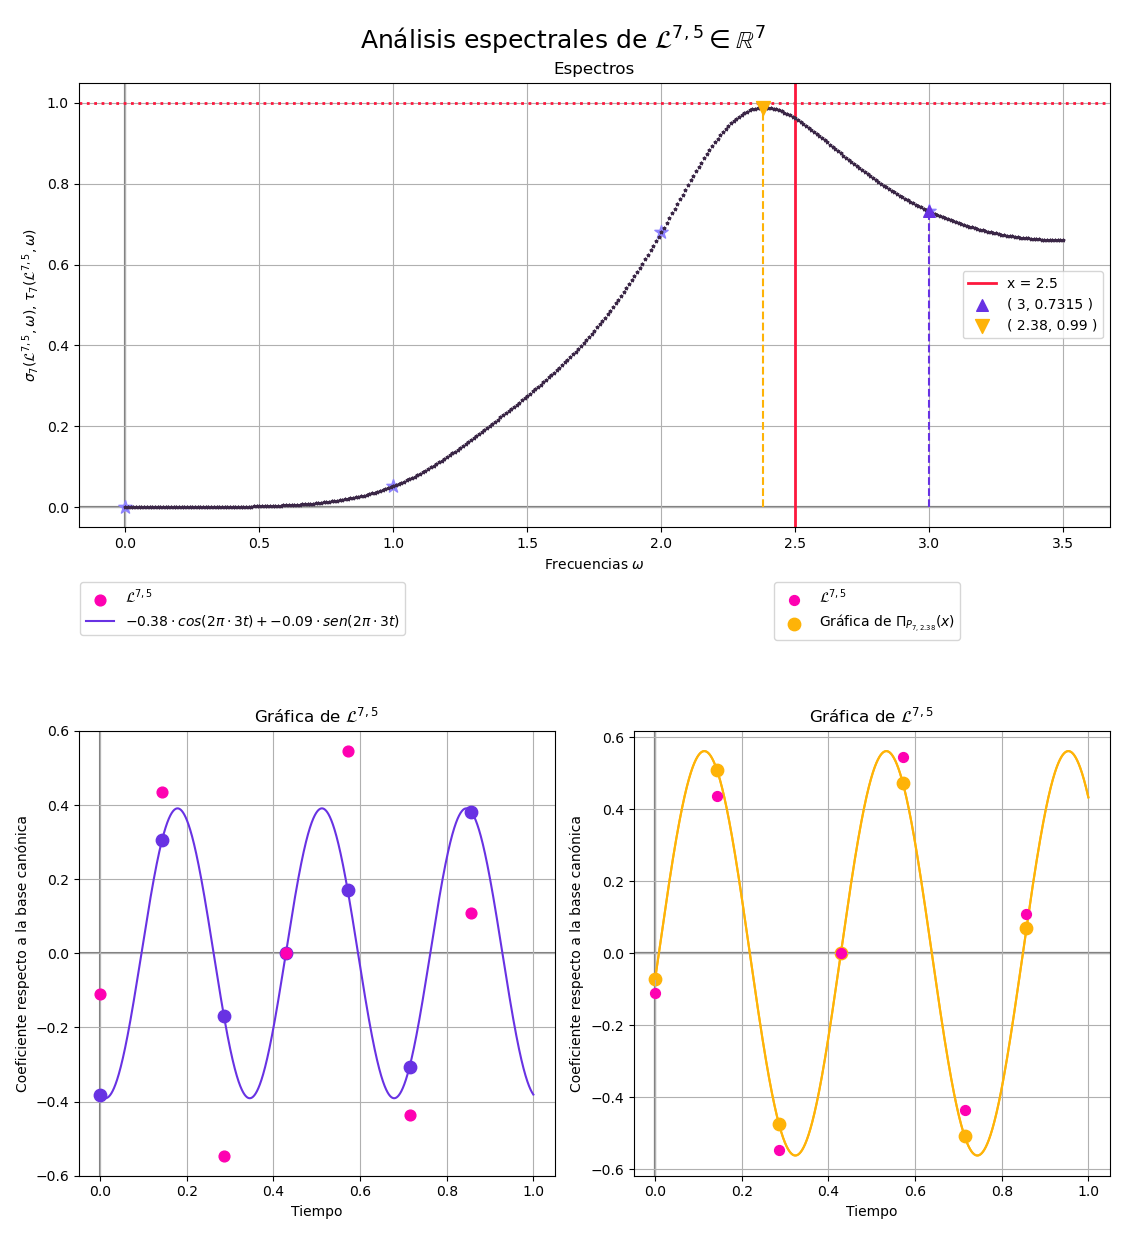
\includegraphics[scale = 0.3]{./graficas_analisisEspectrales/7_5} 
\end{figure}	


\begin{figure}[H]
	\sidecaption{
	\label{fig: 7_6}
	}
	\centering
	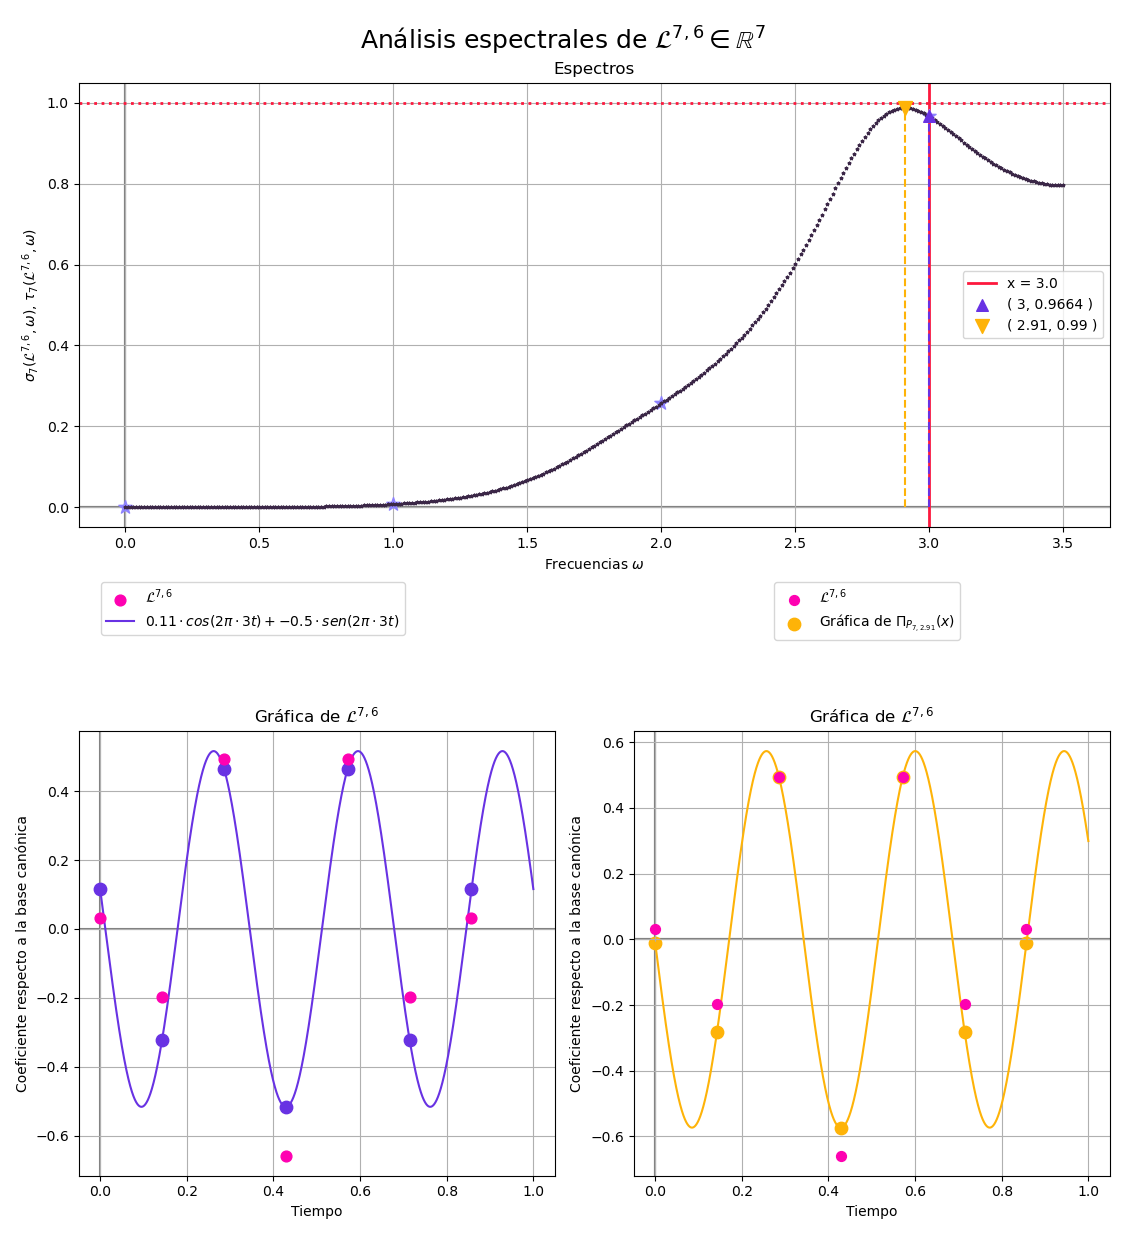
\includegraphics[scale = 0.3]{./graficas_analisisEspectrales/7_6} 
\end{figure}	

A continuación mostramos las gráficas de los puntos
de la forma $(k, FP0(\cali{L}^{7,k}))$
y $(k, FP0(\cali{L}^{7,k}))$.
\begin{figure}[H]
	\sidecaption{
	Observe que $FP0(\cali{L}^{7,0}) = 0 = FP1(\cali{L}^{7,0})$
	pero $FP0(\cali{L}^{7,1}) = 1 $ mientras que 
	$FP1(\cali{L}^{7,1})$, aunque no es cero, es un decimal muy cercano
	a cero; observe en la figura \ref{fig: 7_1}, donde se dibuja
	el espectro de $\cali{L}^{7,1}$ que, en efecto,
	usando un sinusoide de frecuencia 
	$0.01$ (la dada por el espectro
	basado en espacios monofrecuenciales), 
	logramos ajustar casi a la perfección la gráfica de $\cali{L}^{7,1}$
	(que, según el teorema \ref{cor: BON de legendre para espacios Wk}, yace
	en una recta, por lo que no puede ser ajustada a la perfección por un
	sinusoide),
	mientras que usando un sinusoide de frecuencia $1$ (la dada por el 
	espectro basado en la TDF), no se logran ajustar tan bien los datos.
	\label{fig: 7}
	}
	\centering
	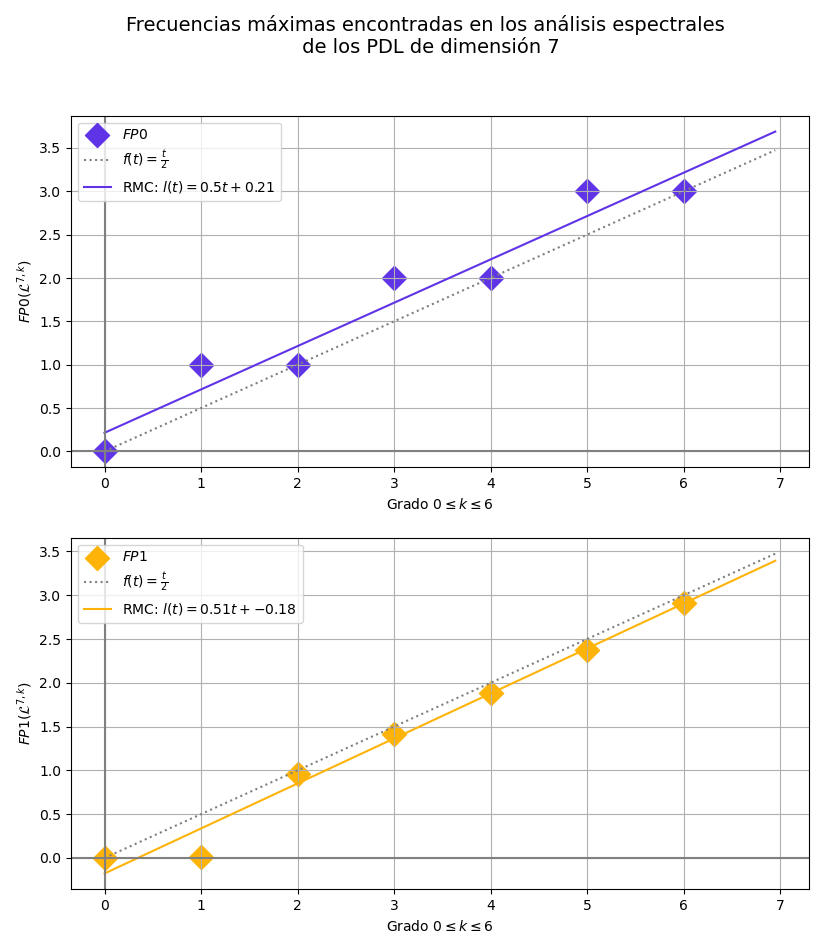
\includegraphics[scale = 0.33]{./estudios_espectrales/7} 
\end{figure}	

Como notamos en la descripción de la figura
\ref{fig: 7}, parece ser que usando el estudio espectral basado en 
espacios monofrecuenciales obtenemos una aproximación de la gráfica
de $\cali{L}^{n,1}$, con $n=7$, en base a un sinusoide de frecuencia muy baja;
grafiquemos 
los puntos de la forma
\eqref{eq0: 8may} y \eqref{eq1: 8may} para 
$k=1$
para ver si esta es una particularidad de la dimensión
$n=7$ o si también ocurre para otros valores de $n$.

\begin{figure}[H]
	\sidecaption{
	Comprobamos numéricamente que los resultados del espectro-1
	sugieren usar frecuencias muy bajas para modelar los 
	PDL de grado $1$; la única excepción se da para $n=3$. Graficamos
	a continuación, en la figura 
	\ref{fig: 3_1},
	los espectros de $\cali{L}^{3,1}$ para ver qué
	está sucediendo.
	\label{fig: k_1}
	}
	\centering
	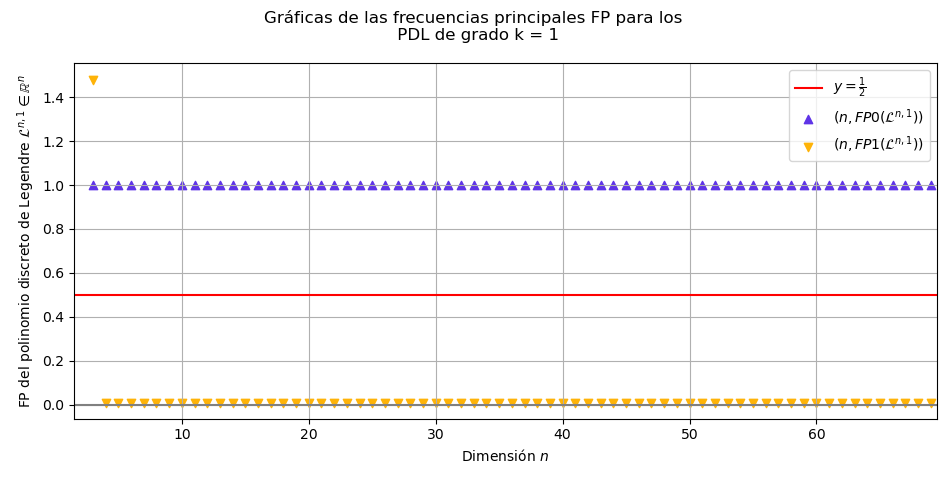
\includegraphics[scale = 0.5]{./estudios_espectrales/k_1} 
\end{figure}	


\begin{figure}[H]
	\sidecaption{
	Como se muestra en los espectros, el coeficiente
	$\sigma_{3}(\mathcal{L}^{3,1}, \omega)$ es, para casi toda
	$\omega$ considerada, muy cercana a uno, por lo que cualquiera
	de estas frecuencias sería adecuada para aproximar con un sinusoide la 
	gráfica de $\mathcal{L}^{3,1}$. Por la forma en que programamos
	el proceso, se usa la última frecuencia más alta, que resultó ser
	$1.48$. Como puede comprobar en las gráficas de abajo, se puede
	aproximar bien la gráfica de $\mathcal{L}^{3,1}$ tanto
	con frecuencia $\omega = 1$ como con frecuencia
	$\omega = 1.48$.
	\label{fig: 3_1}
	}
	\centering
	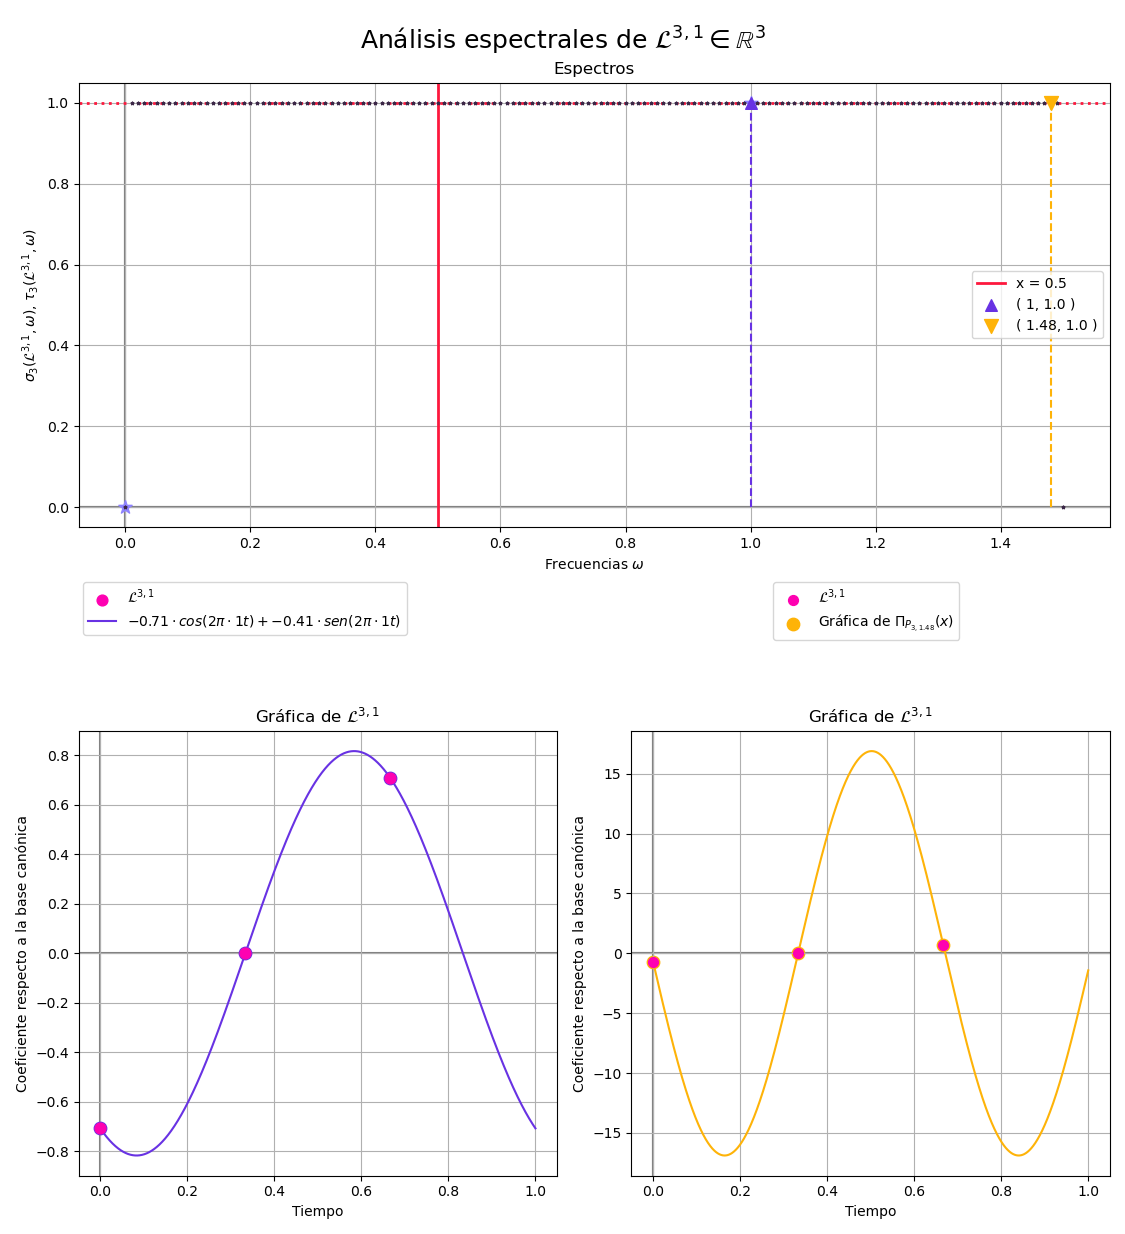
\includegraphics[scale = 0.45]{./estudios_espectrales/3_1} 
\end{figure}	

Comprobemos, graficando los espectros 
de algunos PDL de grado $1$ y dimensión mayor a $3$, 
que frecuencias muy cercanas a $0$ son buenas para modelar
la gráfica de $\cali{L}^{n,1}$, hecho que es 
sugerido por la figura \ref{fig: k_1}.

\begin{figure}[H]
	\sidecaption{
	Note que en este espectro no ocurre lo que se tenía
	en el del PDL $\cali{L}^{3,1}$ (c.f. figura 
	\ref{fig: 3_1}); en este caso, el espectro-$1$ muestra
	claramente que $\omega =0.1$, la frecuencia considerada
	en el análisis
	más cercana a $0$ que \textbf{no} es cero, es la mejor
	(en el sentido explicado en la nota 
	\ref{nota: la mejor frecuencia}).
	\label{fig: 8_1}
	}
	\centering
	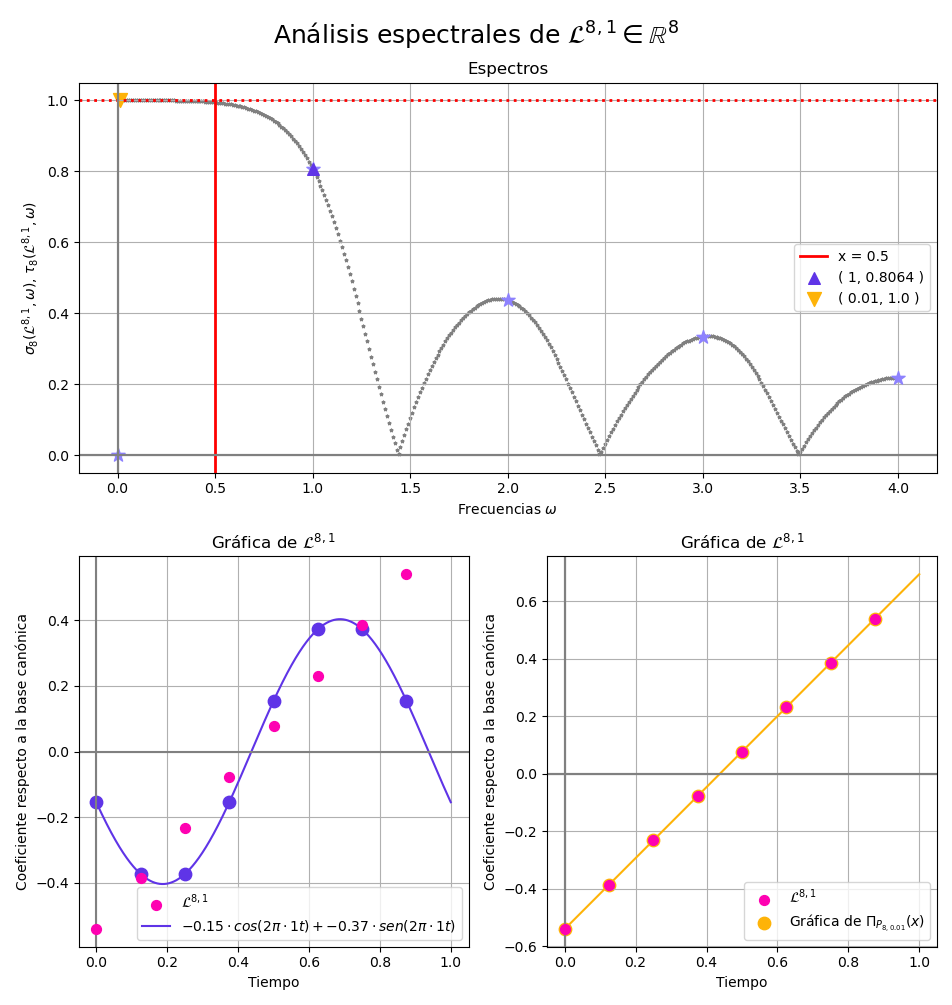
\includegraphics[scale = 0.45]{./estudios_espectrales/8_1} 
\end{figure}	

\begin{figure}[H]
	\sidecaption{
	}
	\centering
	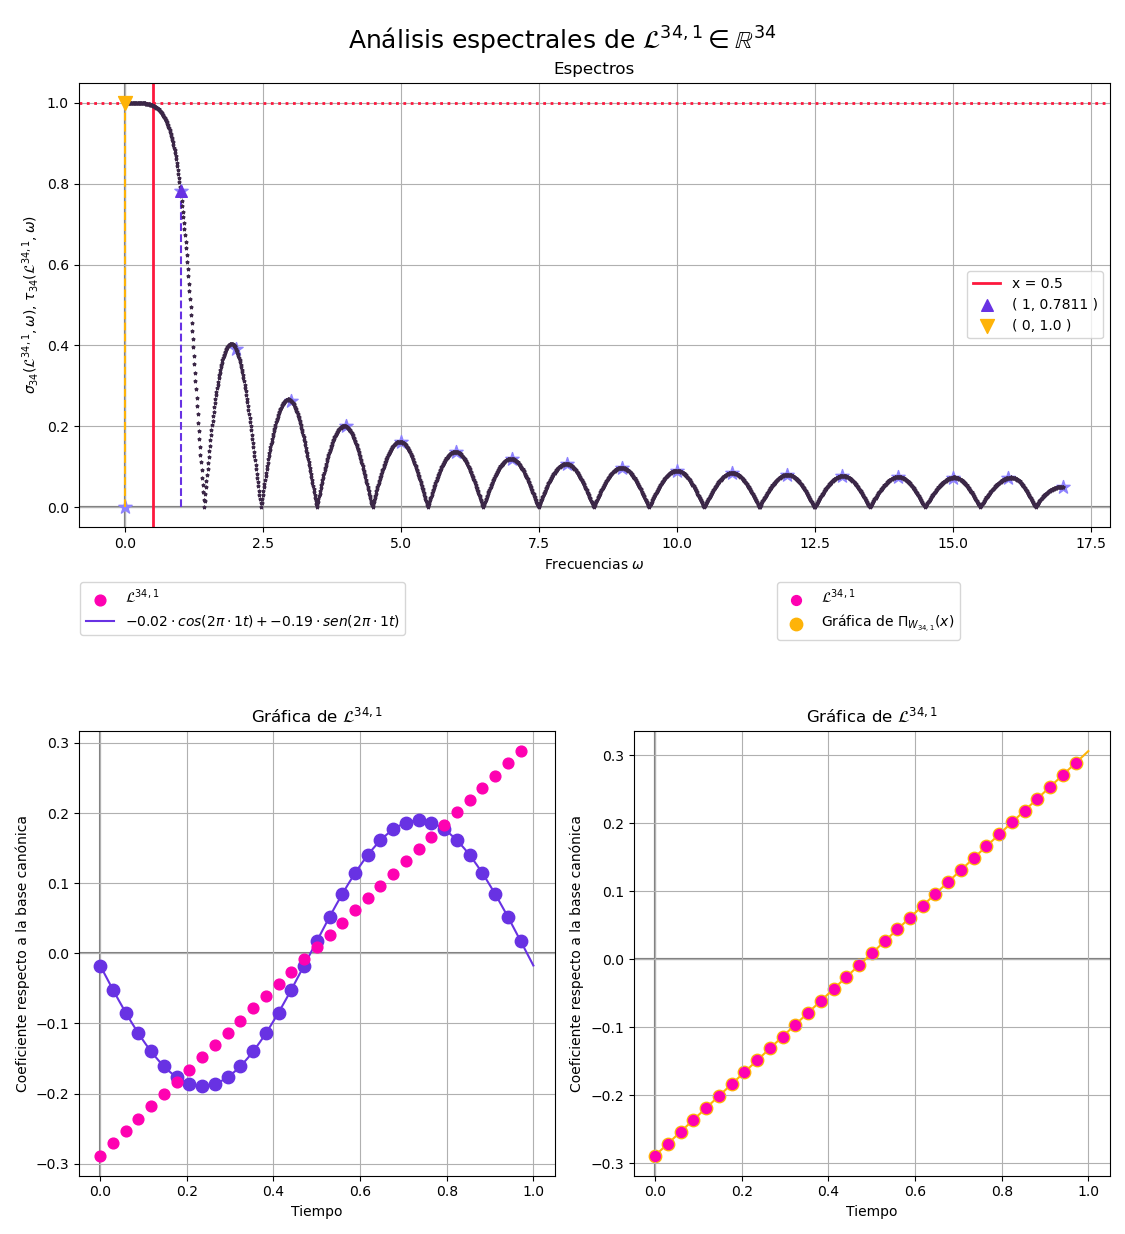
\includegraphics[scale = 0.45]{./estudios_espectrales/34_1} 
\end{figure}	

Puede comprobar, mirando los espectros
de los PDL $\cali{L}^{n,1}$ de grado $1$,
que siempre se tiene que $ \omega = 0.01$ es la frecuencia
que maximiza el coeficiente espectral
$\sigma_{n}(\cali{L}^{n,k}, \omega)$.
Esto se explica observando que
lo que estamos haciendo con este análisis espectral
es aproximar las gráficas de señales con sinusoides, que son
funciones diferenciables en todo punto
(hecho que puede
puede interpretarse
como que los ``alrededores
cercanos'' de cualquier
punto de la gráfica de un sinusoide son 
parecidos a una recta), luego, tiene sentido que  
el análisis espectral de mayor peso a las 
frecuencias cercanas a cero
para modelar la gráfica de $\cali{L}^{n,k}$
que, según el teorema 
\ref{cor: BON de legendre para espacios Wk}, está contenida
en una recta. Observe que 
$\sigma_{n}(\cali{L}^{n,k}, 0)$ es cero, pues
$P_{n, 0}$ está generado por
$c_{n,0}$, que es el vector constante uno, y que 
es ortogonal a $\cali{L}^{n,k}$. Así, los espectros
de los PDL de grado $1$ tienen una discontinuidad de salto
por la derecha del cero. \\


Graficando algunos PDL de dimensión
39, apreciamos que conforme $k$ aumenta, es menos
sencillo aproximar la gráfica del respectivo PDL
con un solo sinusoide.
\begin{figure}[H]
	\sidecaption{
	}
	\centering
	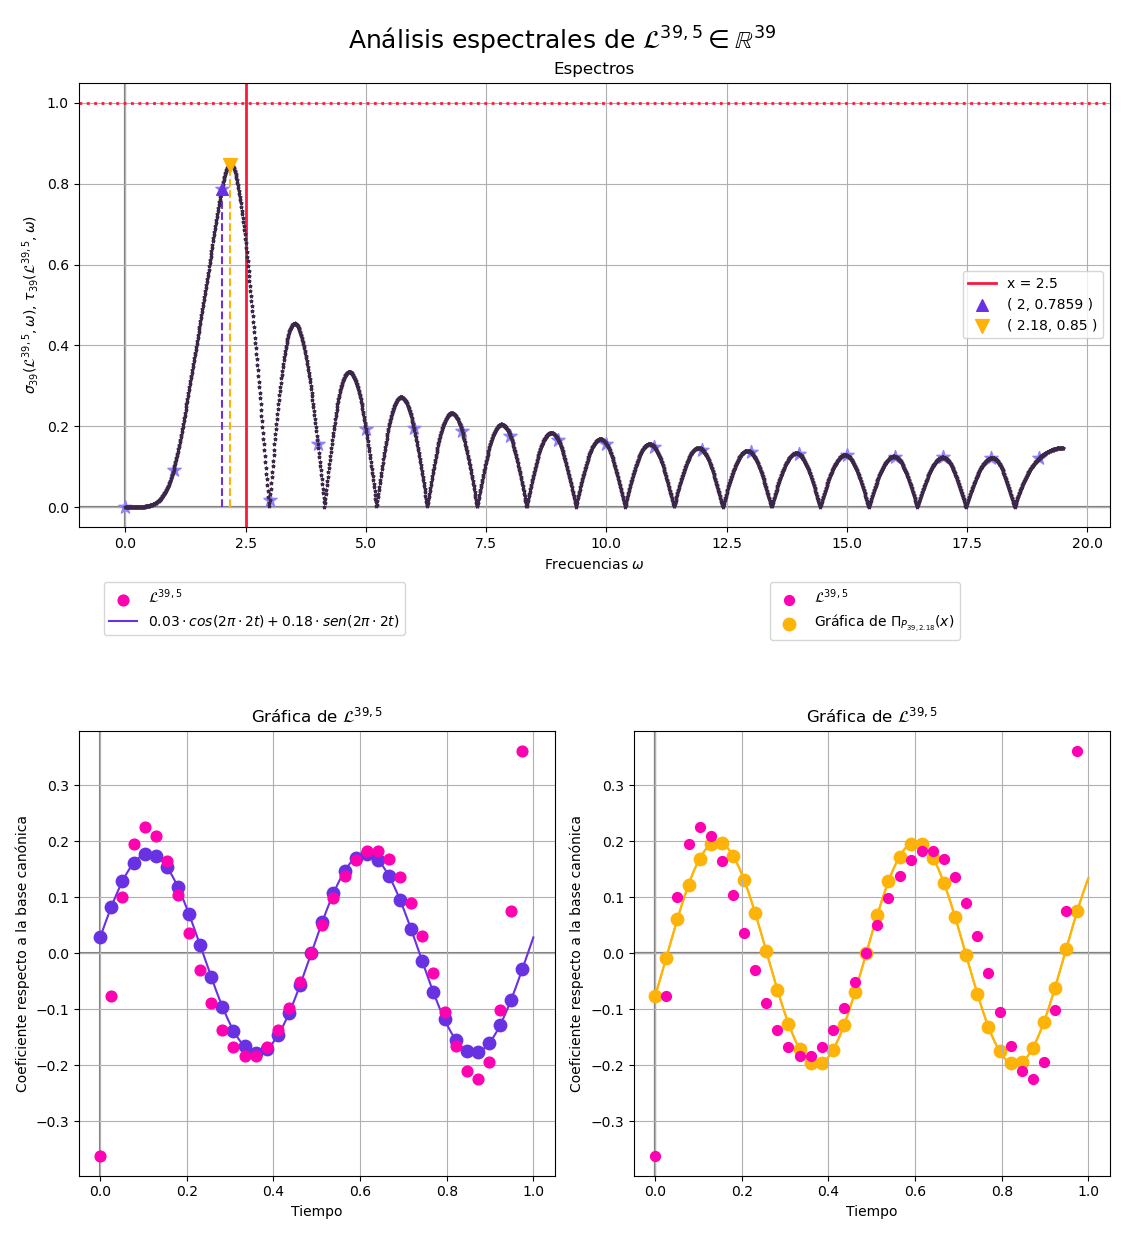
\includegraphics[scale = 0.45]{./estudios_espectrales/39_5} 
\end{figure}	
\begin{figure}[H]
	\sidecaption{
	}
	\centering
	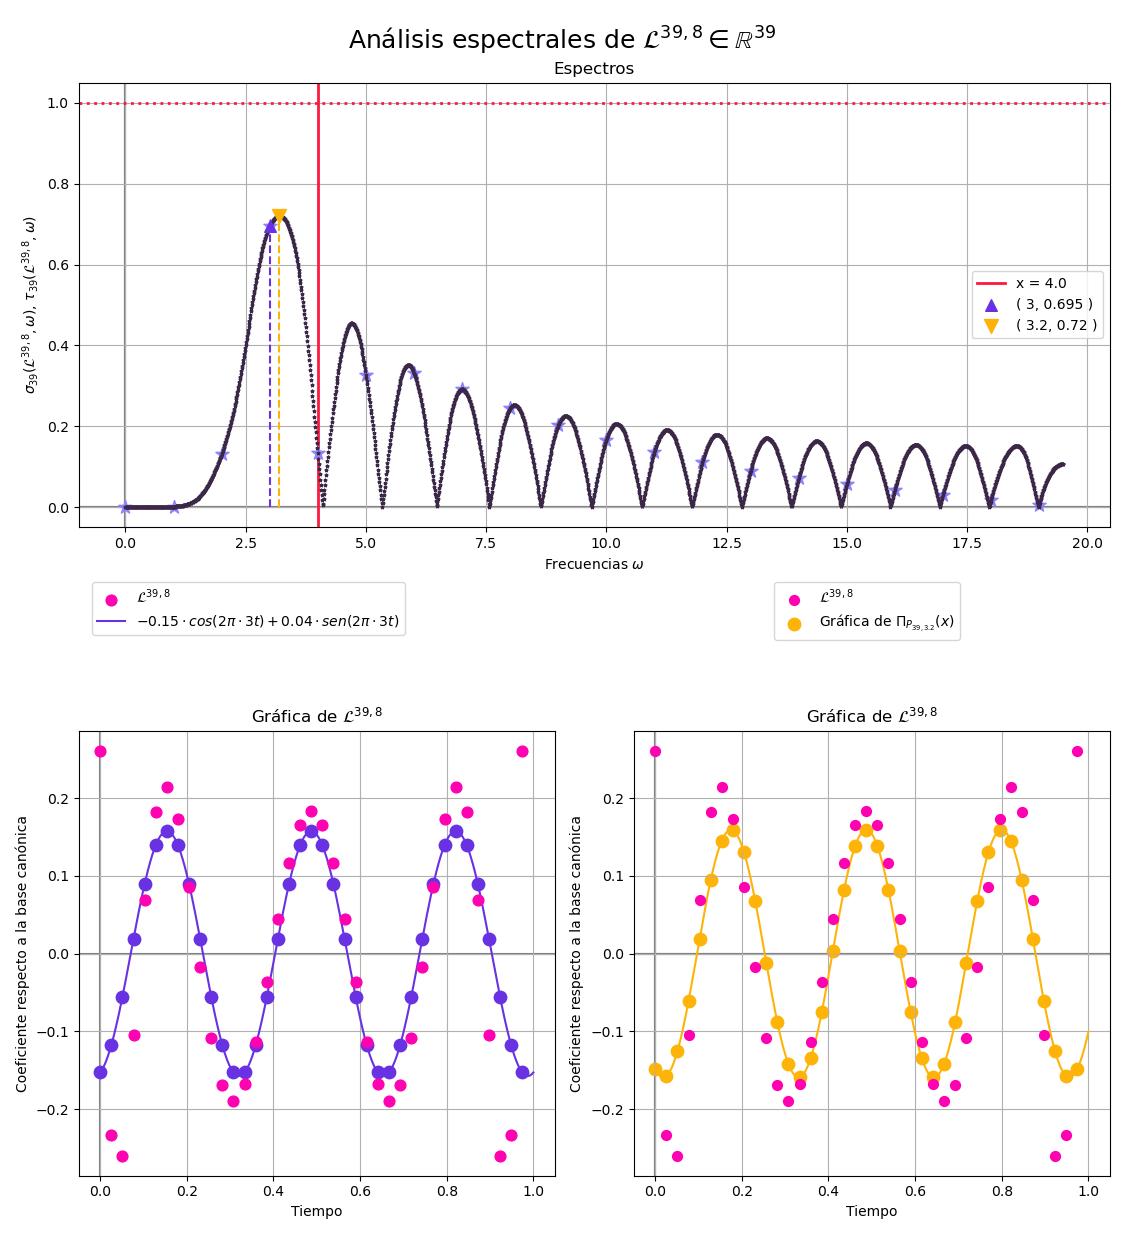
\includegraphics[scale = 0.45]{./estudios_espectrales/39_8} 
\end{figure}	
\begin{figure}[H]
	\sidecaption{
	}
	\centering
	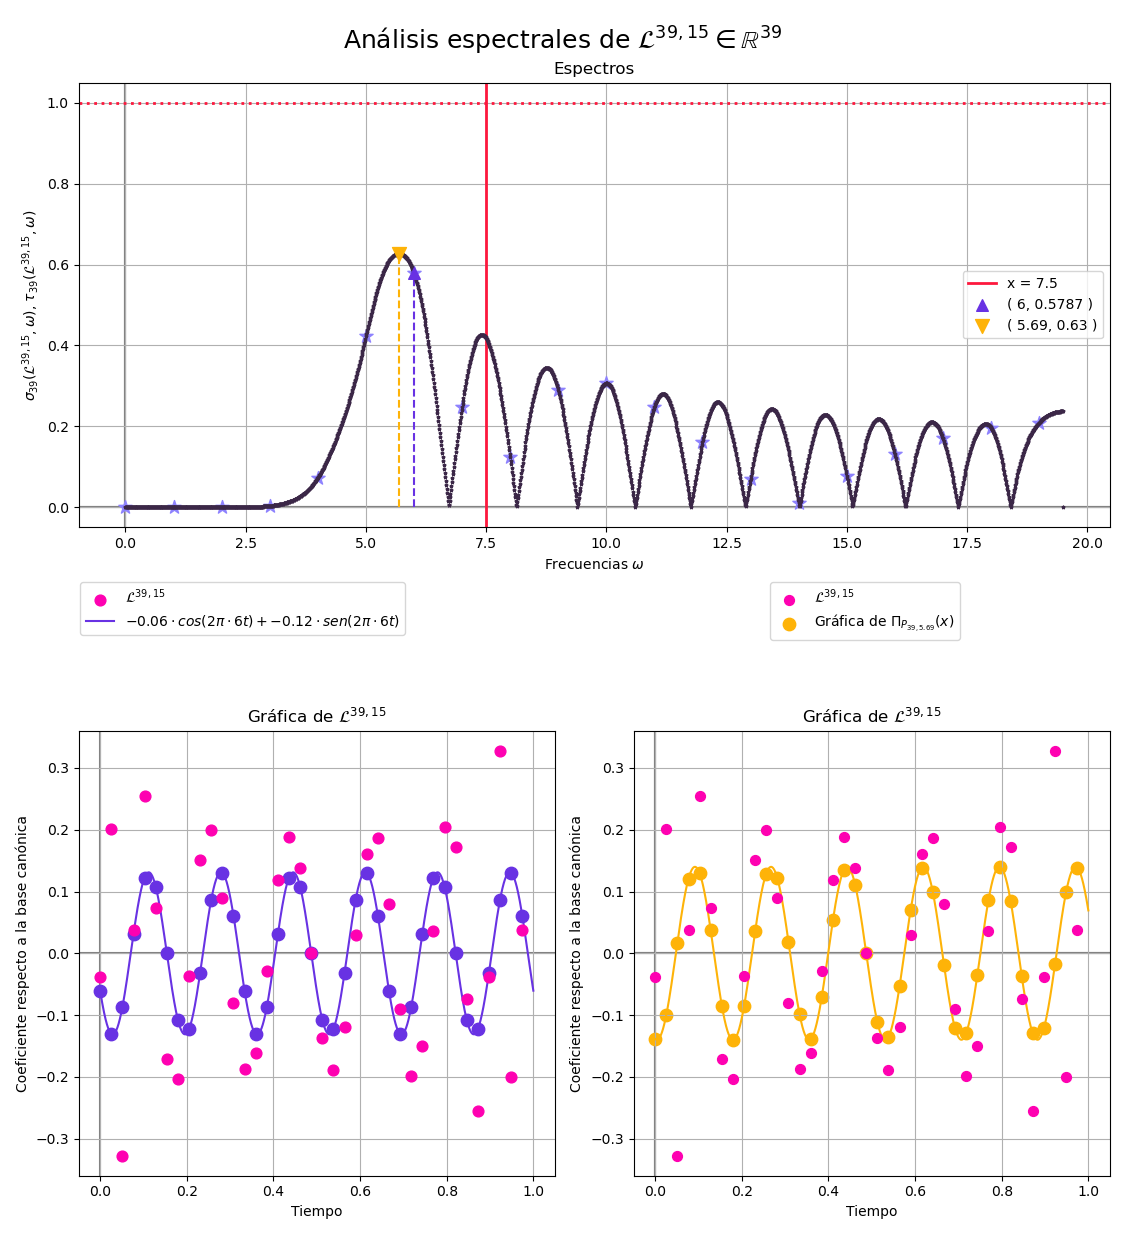
\includegraphics[scale = 0.45]{./estudios_espectrales/39_15} 
\end{figure}	
\begin{figure}[H]
	\sidecaption{
	}
	\centering
	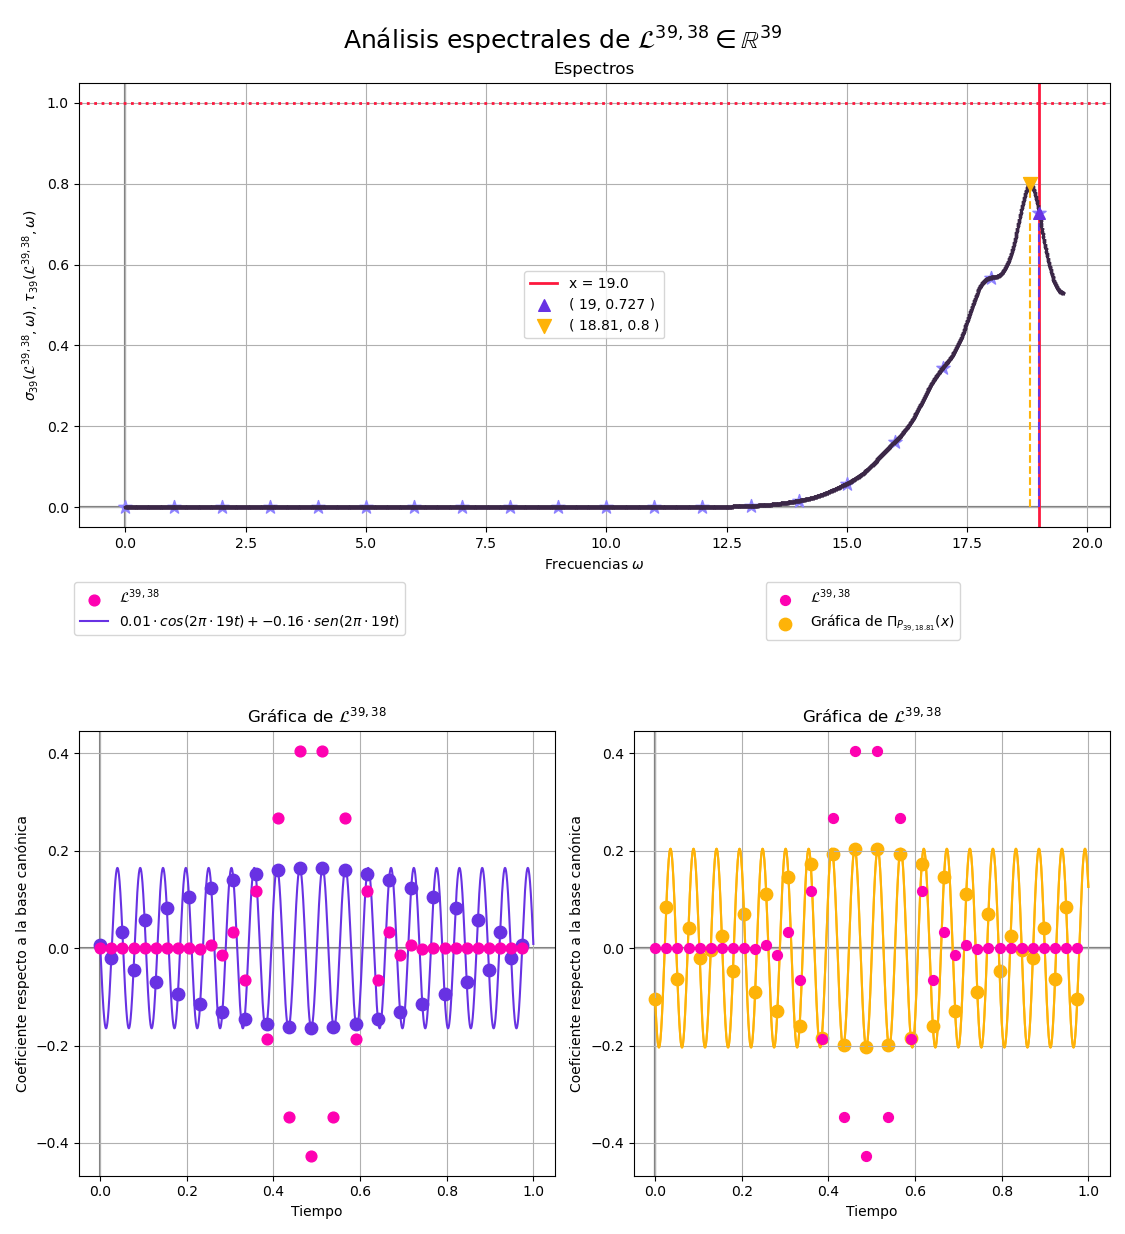
\includegraphics[scale = 0.25]{./estudios_espectrales/39_38} 
\end{figure}	

Sin embargo, puede observar en los espectros guardados en 
\TODO{referencia a carpeta} que, para las dimensiones consideradas,
se consigue aproximar muy bien la gráfica del PDL
$\cali{L}^{n,k}$ cuando $k$ es cercano a cero, y además 
que los espectros parecen tener un solo máximo global
(i.e. una sola frecuencia principal 
$\omega \in \left[0, \frac{n}{2} \right]$).

Graficando algunos conjuntos de puntos
de la forma
$(k, FP0(\cali{L}^{n,k}))$ y 
$(k, FP1(\cali{L}^{n,k}))$ para ciertas
dimensiones $n$, veamos si, como 
afirmamos en la hipótesis 
\ref{ref: hipotesis}, la frecuencia principal
resultante de tales análisis es cercana
a $\frac{k}{2}$.

\begin{figure}[H]
	\sidecaption{
	Estudio de frecuencias principales
	para dimensión $n = 9$.
	Las ecuaciones de las rectas de mínimos
	cuadrados para los dos análisis son
	$l_{9, 0}(t) = 0.45t + 0.09$ y 
	$l_{9, 1}(t) = 0.5t -0.18$.
	\label{fig: n 9}
	}
	\centering
	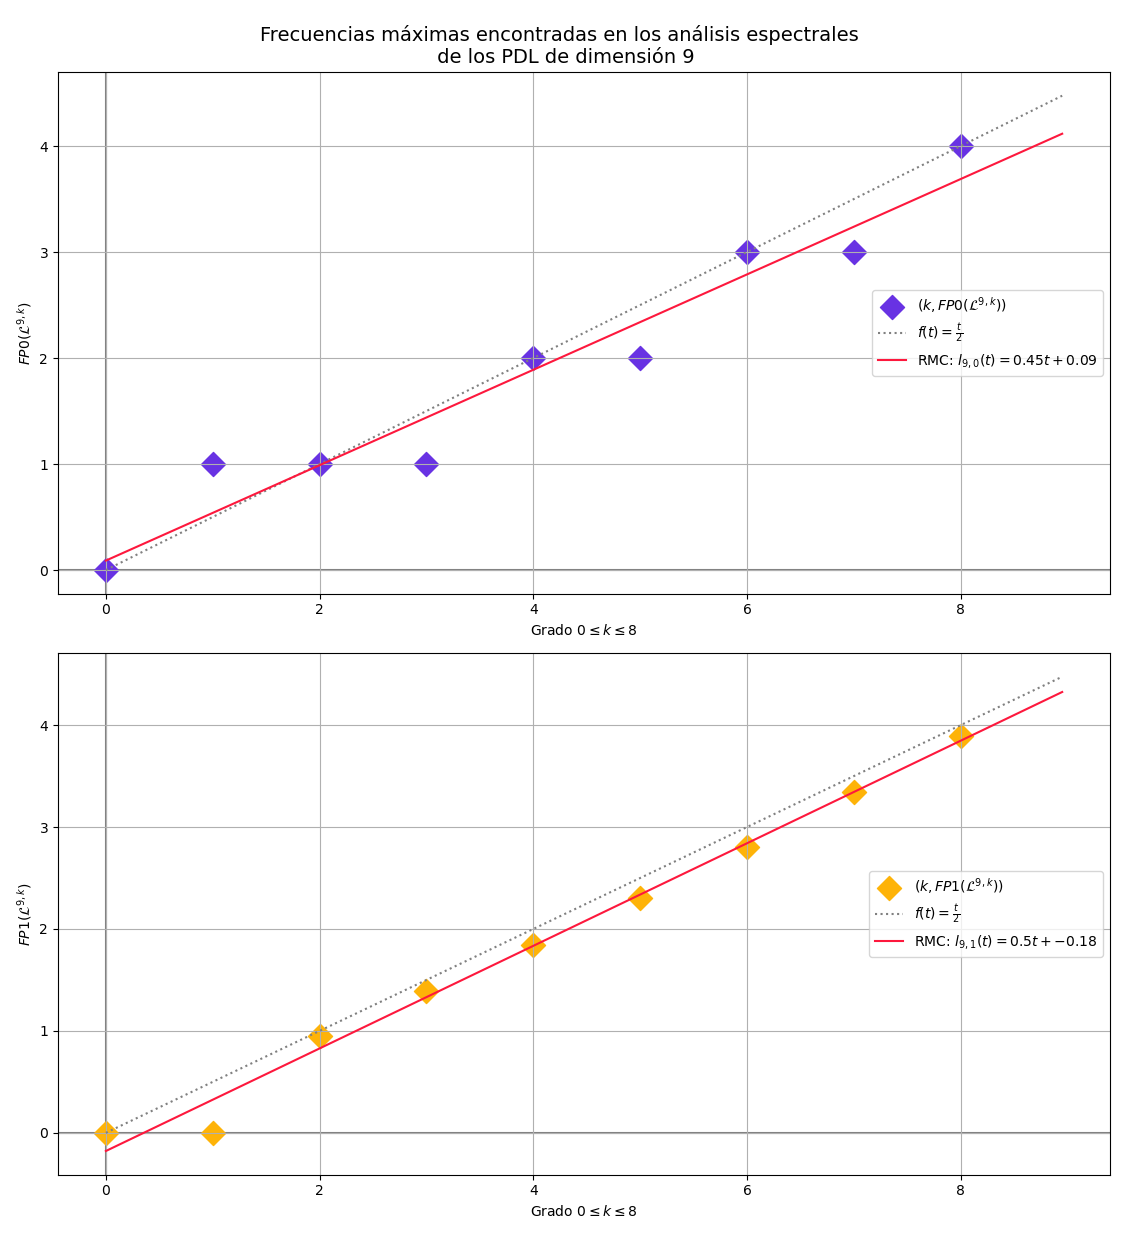
\includegraphics[scale = 0.3]{./graficas_analisisEspectrales/n_9} 
\end{figure}	

\begin{figure}[H]
	\sidecaption{
	Estudio de frecuencias principales
	para dimensión $n = 20$.
	Las ecuaciones de las rectas de mínimos
	cuadrados para los dos análisis son
	$l_{20, 0}(t) = 0.44t -0.04$ y 
	$l_{20, 1}(t) = 0.46t -0.25$.
	\label{fig: n 20}
	}
	\centering
	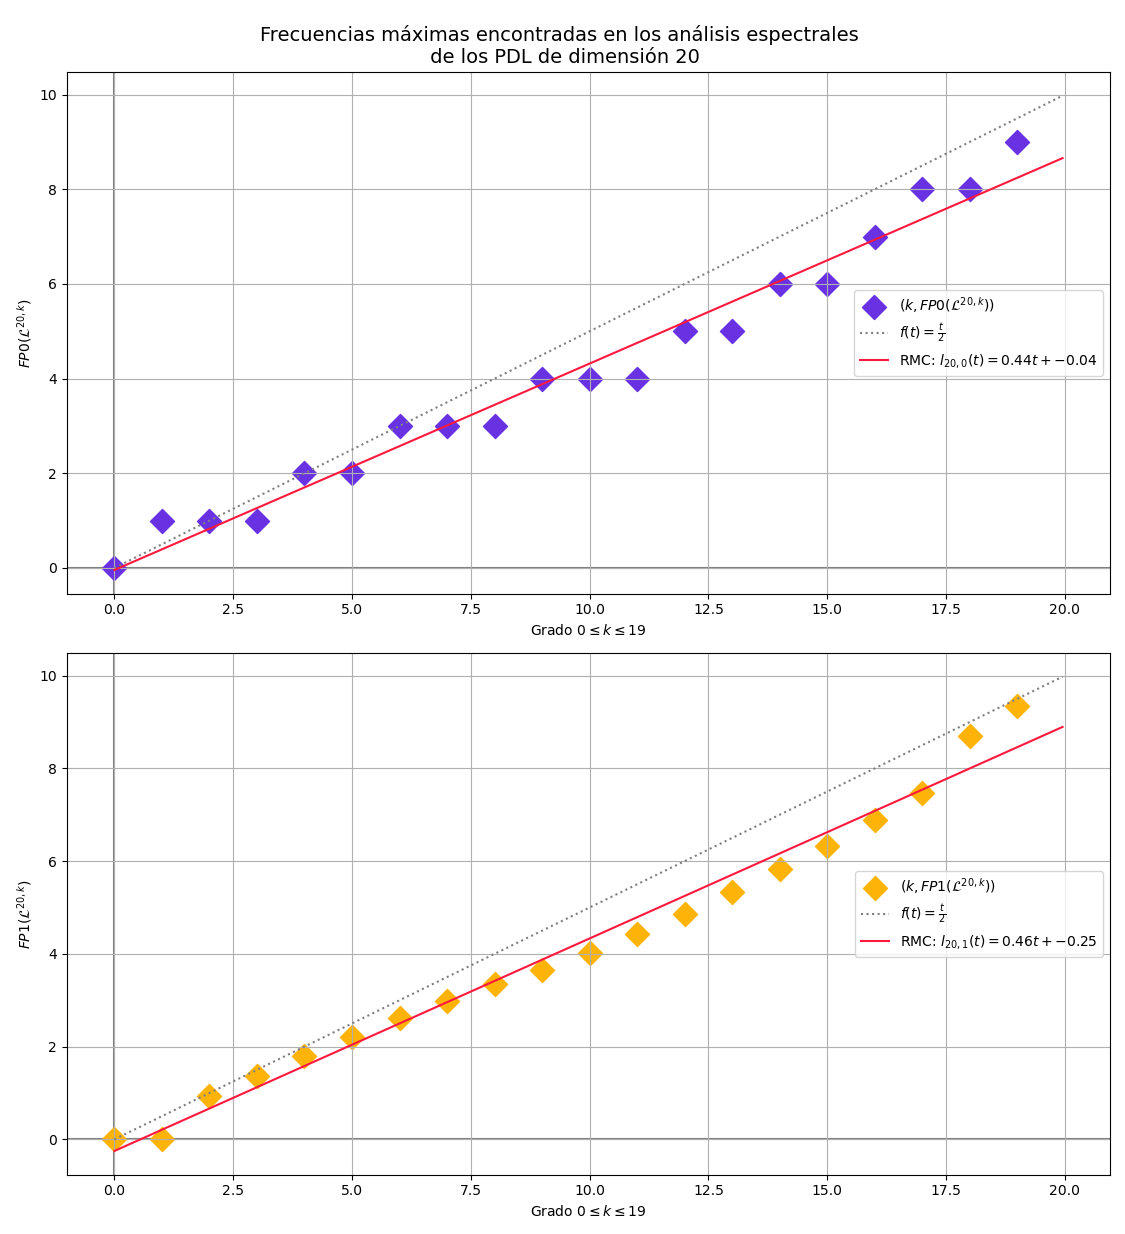
\includegraphics[scale = 0.3]{./graficas_analisisEspectrales/n_20} 
\end{figure}

\begin{figure}[H]
	\sidecaption{
	Estudio de frecuencias principales
	para dimensión $n = 25$.
	Las ecuaciones de las rectas de mínimos
	cuadrados para los dos análisis son
	$l_{25, 0}(t) = 0.45t - 0.26$ y 
	$l_{9, 1}(t) = 0.46t -0.35$.
	\label{fig: n 25}
	}
	\centering
	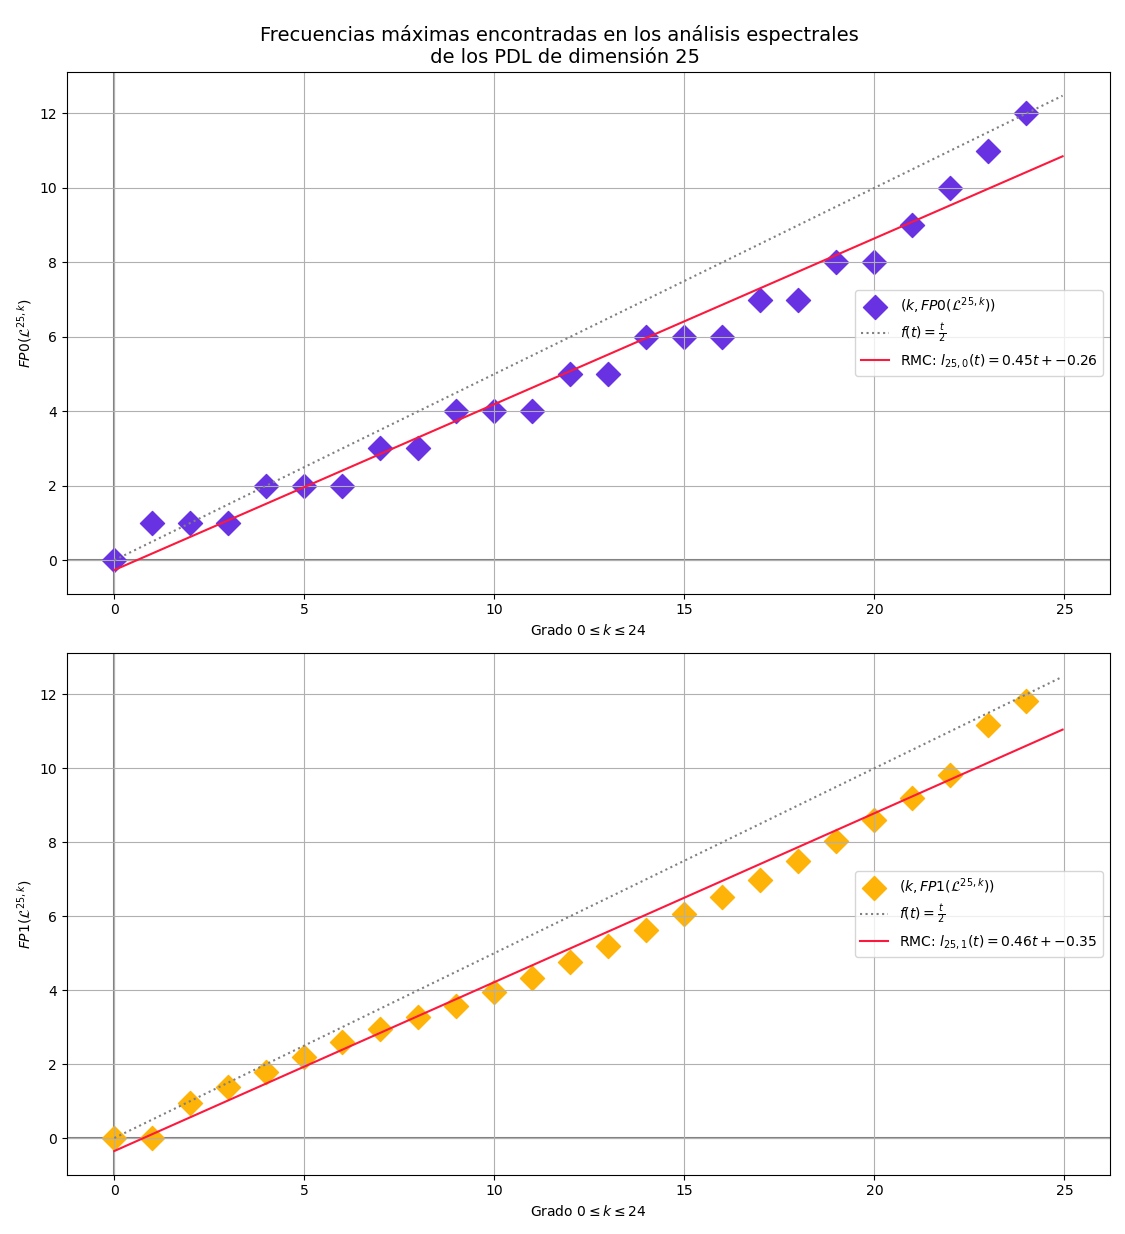
\includegraphics[scale = 0.3]{./graficas_analisisEspectrales/n_25} 
\end{figure}

\begin{figure}[H]
	\sidecaption{
	Estudio de frecuencias principales
	para dimensión $n = 60$.
	Las ecuaciones de las rectas de mínimos
	cuadrados para los dos análisis son
	$l_{60, 0}(t) = 0.43t - 0.98$ y 
	$l_{60, 1}(t) = 0.43t - 1$.
	\label{fig: n 60}
	}
	\centering
	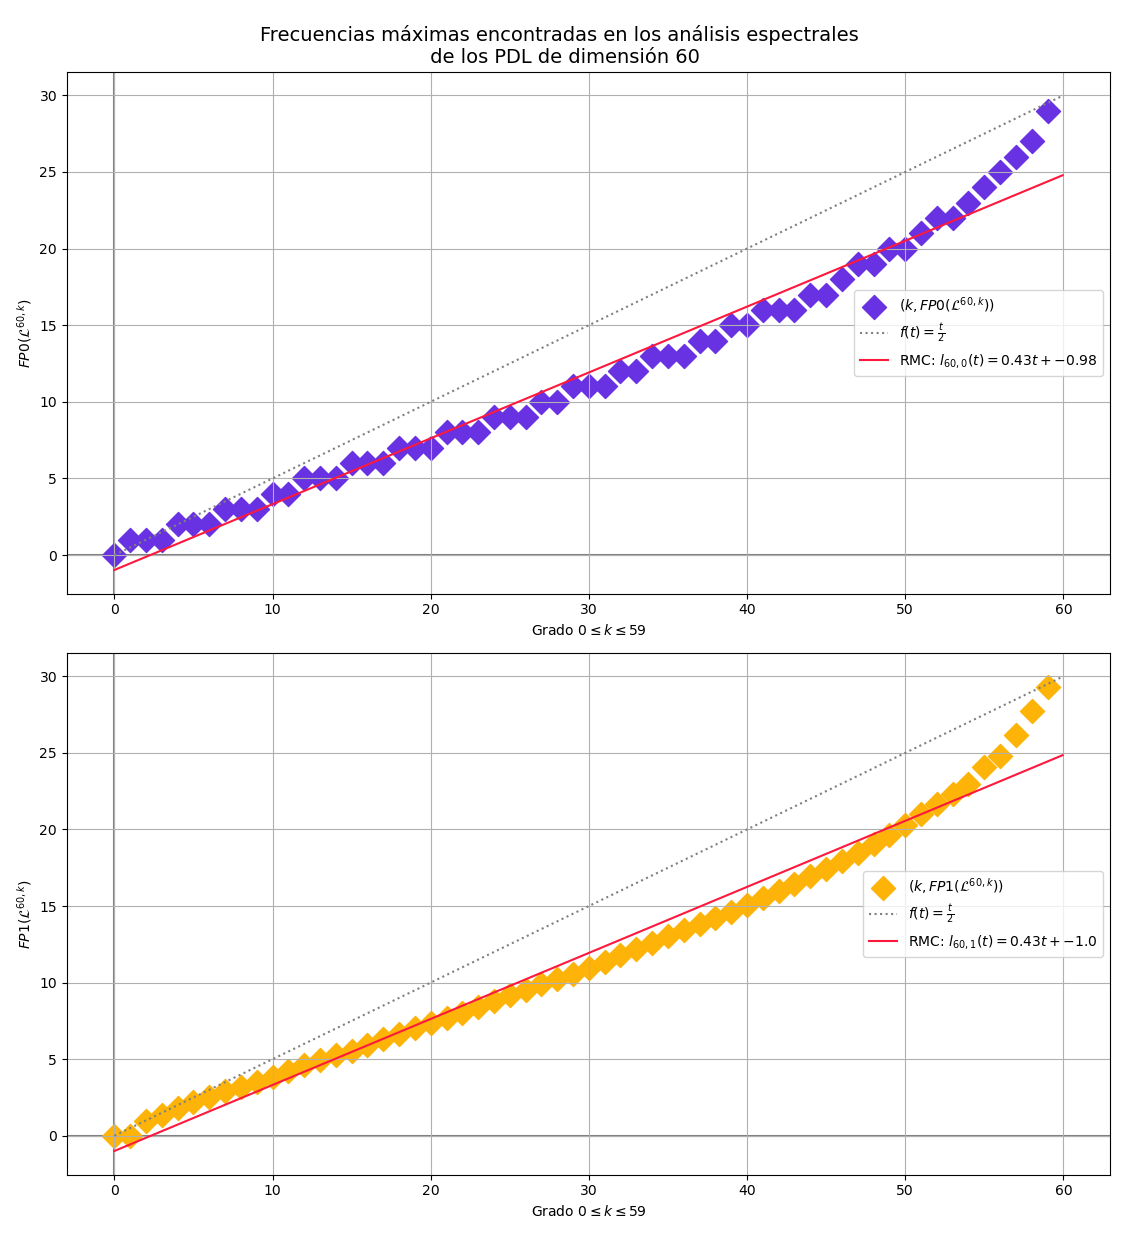
\includegraphics[scale = 0.3]{./graficas_analisisEspectrales/n_60} 
\end{figure}

Parece ser que, conforme $n$ aumenta, la 
pendiente que mejor parece modelar las
frecuencias principales no es
$0.5$ (como afirmamos en nuestra hipótesis), 
sino algo menor, cercana a $0.4$. 
Ya desde el visualizar algunos espectros
de los PDL se percibía que las frecuencias principales
parecían siempre ubicarse a la izquierda de $0.5$.

Grafiquemos los puntos de la forma
$(n, m_{n,0})$, $(n, m_{n,1})$ y 
$(n, b_{n,0})$, $(n, b_{n,1})$ 
para ver si las pendientes de las RMC parecen, como
sugieren las observaciones anteriores, tender a $0.4$,
y qué tendencia parecen seguir las ordenadas al origen.
\begin{figure}[H]
	\sidecaption{
	En esta gráfica comprobamos que las pendientes
	de las rectas de mínimos cuadrados parecen ser más
	bajas que $0.5$ conforme $n$ crece. Para los valores
	de $n$ considerado en estos análisis espectrales,
	vemos que una cota
	inferior para estas pendientes
	es $0.425$. Observe que las ordenadas al origen
	también descienden; si nuestra hipótesis
	\ref{ref: hipotesis} hubiese sido cierta, tales
	ordenadas al origen debería permanecer cerca del cero.
	Con color morado se han graficado los datos
	correspondientes a los análisis realizados
	con la TDF, y se uso un naranja para los de
	los análisis basados en espacios
	monofrecuenciales. Observe que, por lo general, 
	los resultados dados por ambos análisis son parecidos.
	\label{fig: coef RMC}
	}
	\centering
	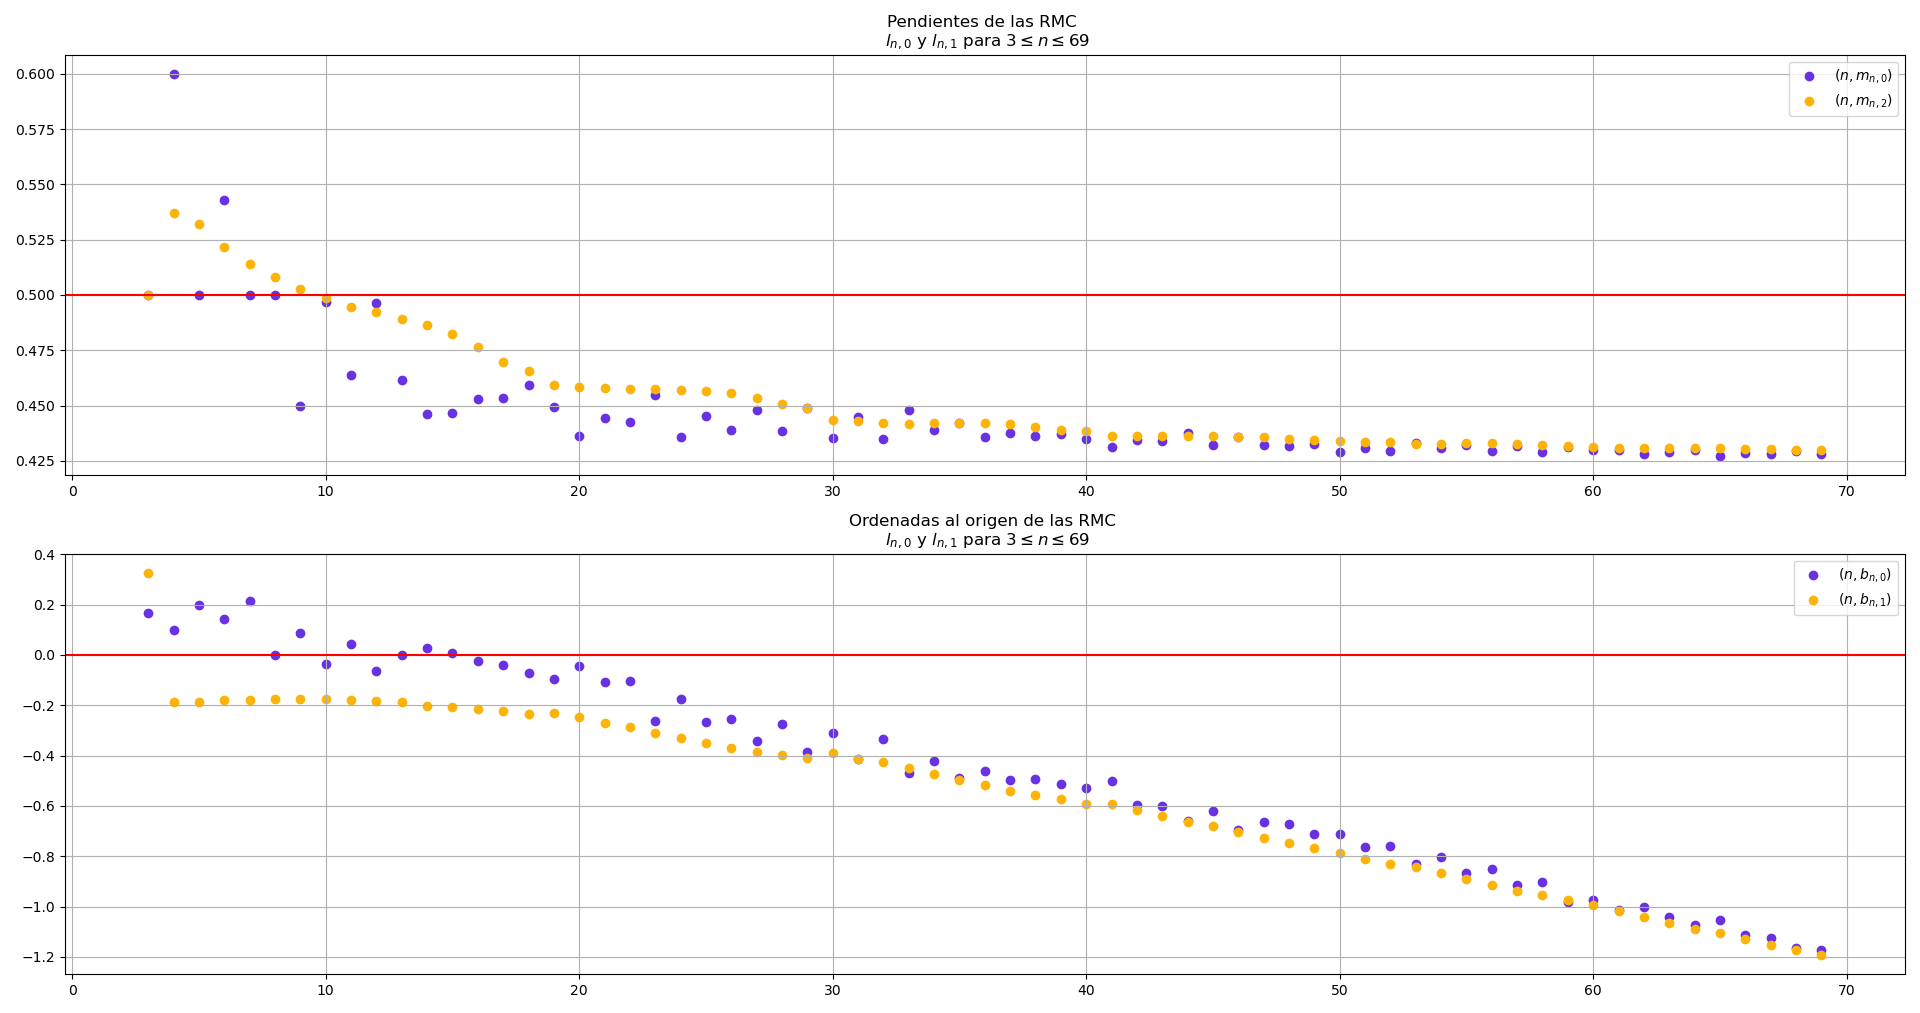
\includegraphics[angle = 90, scale = 0.4]{./estudios_espectrales/graf_coef_RMC} 
\end{figure}	

\begin{figure}[H]
	\sidecaption{
	Aquí la gráfica de las nubes de puntos
	de las que se habló en la figura 
	\ref{fig: ejemplo_pregunta3_1}. Observe que no 
	se acumulan cerca del punto $(0, 0.5)$, como 
	sería de esperar si la respuesta a la pregunta
	\ref{pregunta 1} fuese afirmativa.
	\label{fig: pendiente_oOrigen}
	}
	\centering
	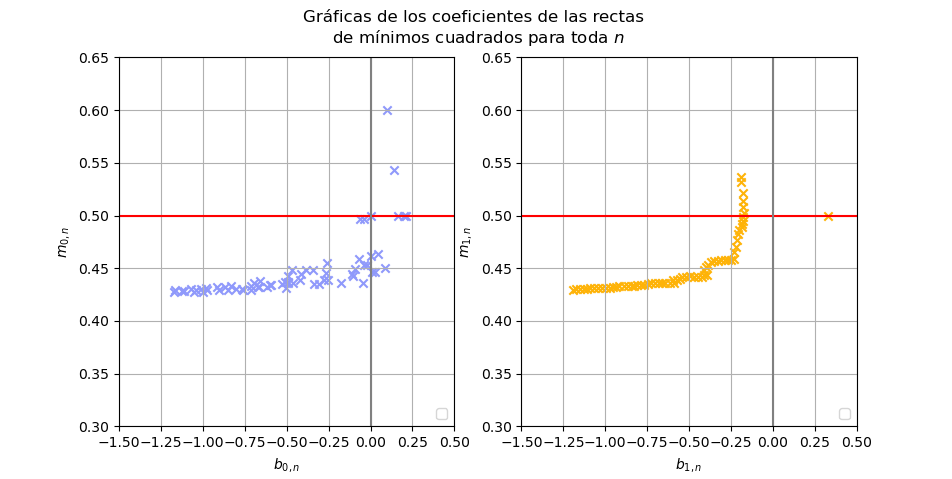
\includegraphics[scale = 0.6]{./estudios_espectrales/pendiente_oOrigen} 
\end{figure}	


Usados ya los parámetros de las rectas
de mínimos cuadrados para
intentar ver si los PDL
de grado $k$ presentan una respuesta
mayor a la frecuencia $k/2$, veamos si al menos
ocurre que la frecuencia principal de
un PDL depende sólo de su parámetro de 
grado $k$, o si también el parámetro
de dimensión $n$ influye. 
Hagamos esto 
fijando un $k \geq 2$ y 
graficando las familias de puntos de la forma
\eqref{eq0: 8may}
y \eqref{eq1: 8may}. Si sólo el parámetro $k$ 
influye en la frecuencia principal, tendríamos graficas
de puntos que siguen una trayectoria horizontal.
Se ha marcado en rojo la recta
$y = \frac{k}{2}$, a la que, según nuestra hipótesis
\ref{ref: hipotesis}, deberían estár cercanos los
puntos de las gráficas. 

\begin{figure}[H]
	\sidecaption{
	\label{fig: k 3}
	}
	\centering
	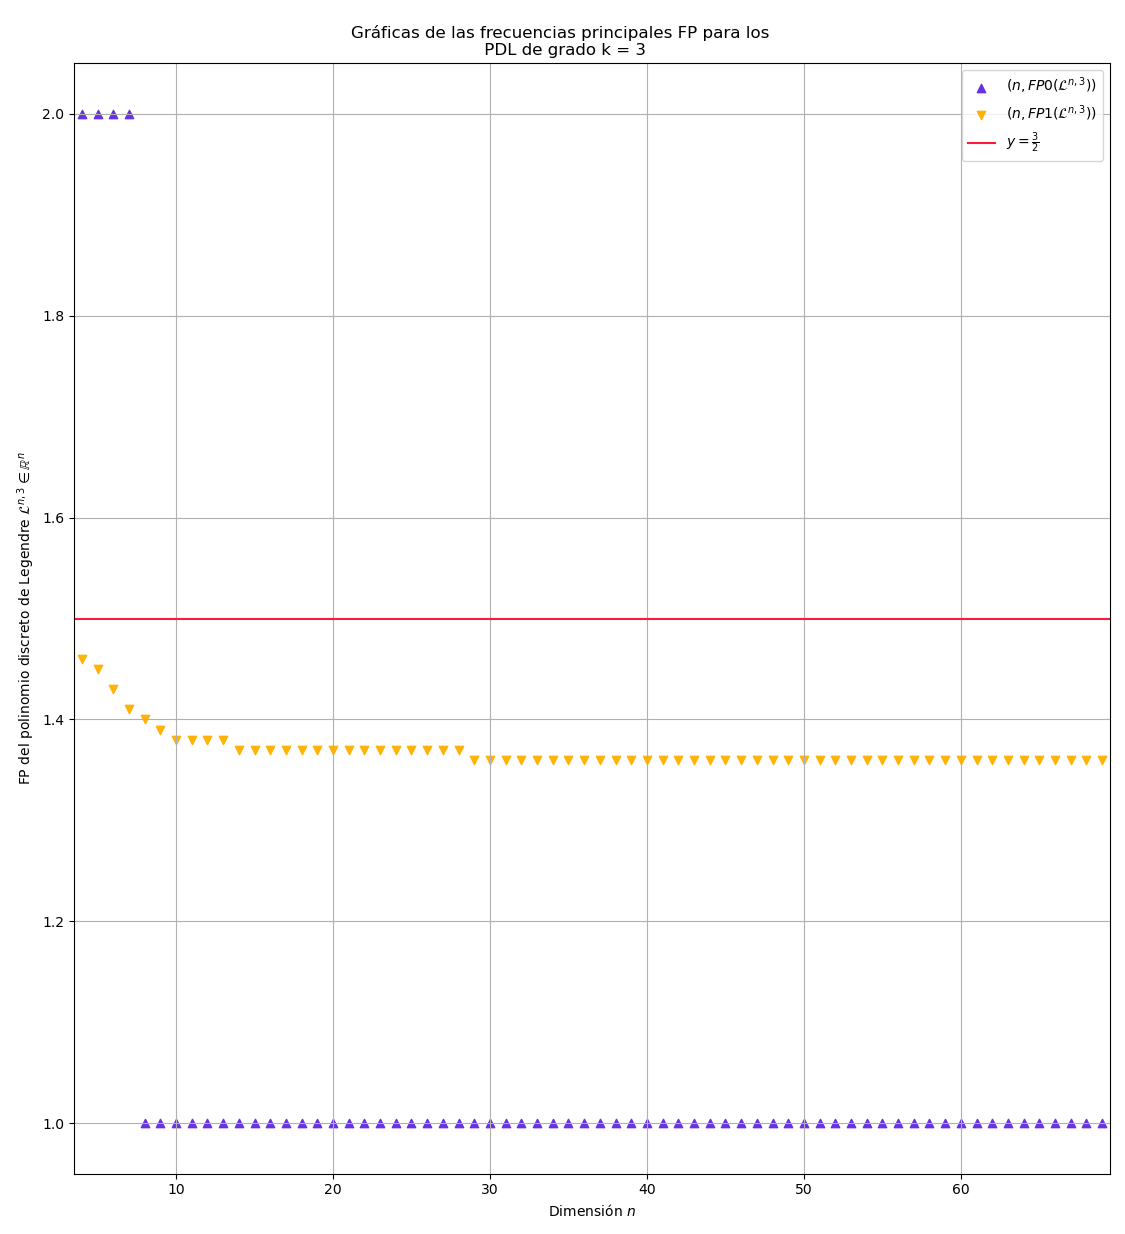
\includegraphics[scale = 0.5]{./estudios_espectrales/k_3} 
\end{figure}

\begin{figure}[H]
	\sidecaption{
	\label{fig: k 8}
	}
	\centering
	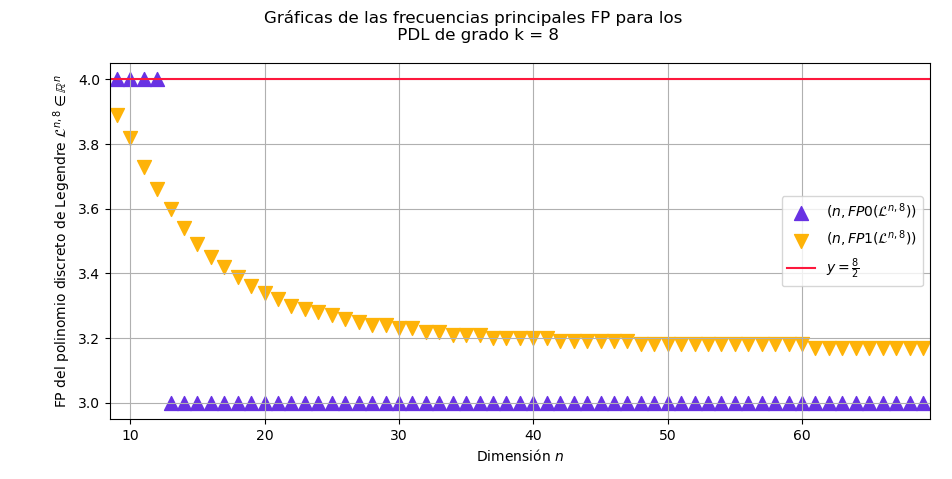
\includegraphics[scale = 0.5]{./estudios_espectrales/k_8} 
\end{figure}

\begin{figure}[H]
	\sidecaption{
	\label{fig: k 10}
	}
	\centering
	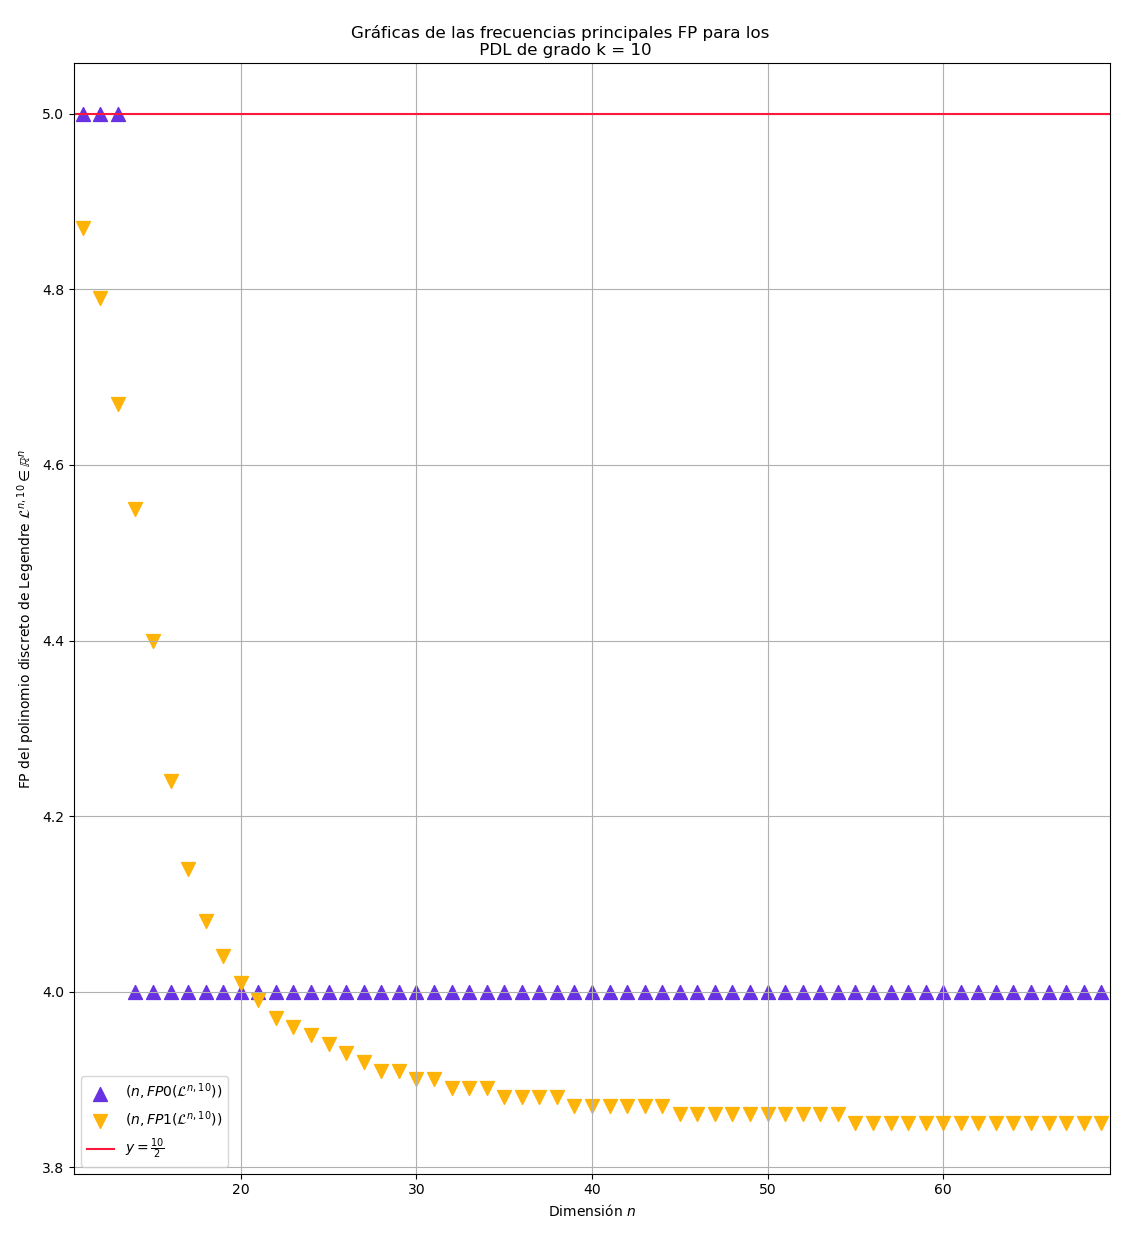
\includegraphics[scale = 0.5]{./estudios_espectrales/k_10} 
\end{figure}

\begin{figure}[H]
	\sidecaption{
	\label{fig: k 16}
	}
	\centering
	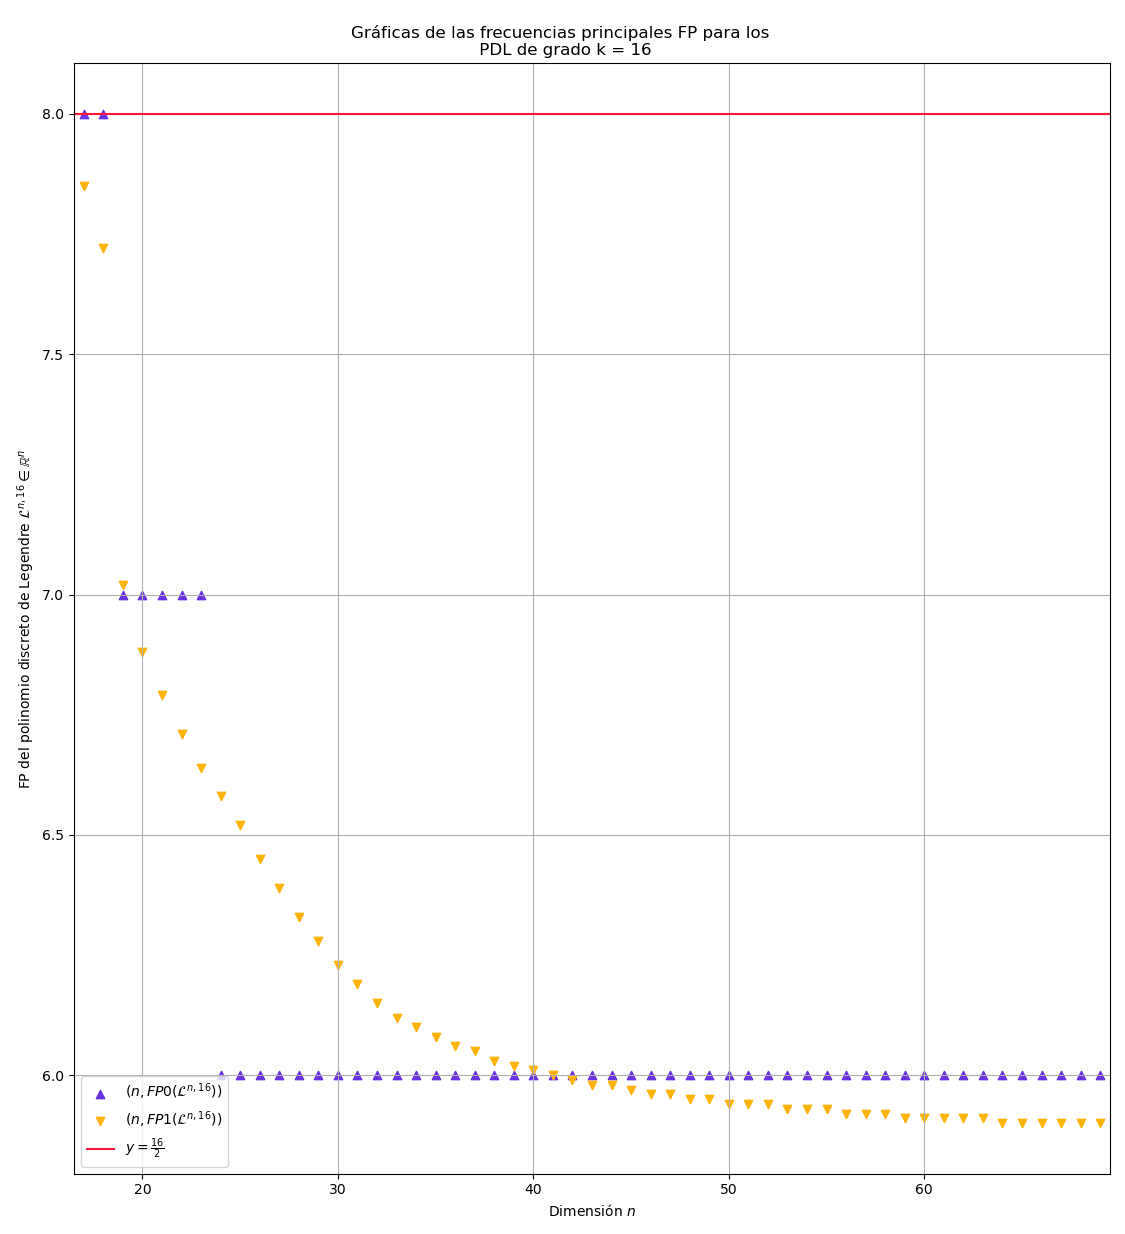
\includegraphics[scale = 0.5]{./estudios_espectrales/k_16} 
\end{figure}

\begin{figure}[H]
	\sidecaption{
	\label{fig: k 20}
	}
	\centering
	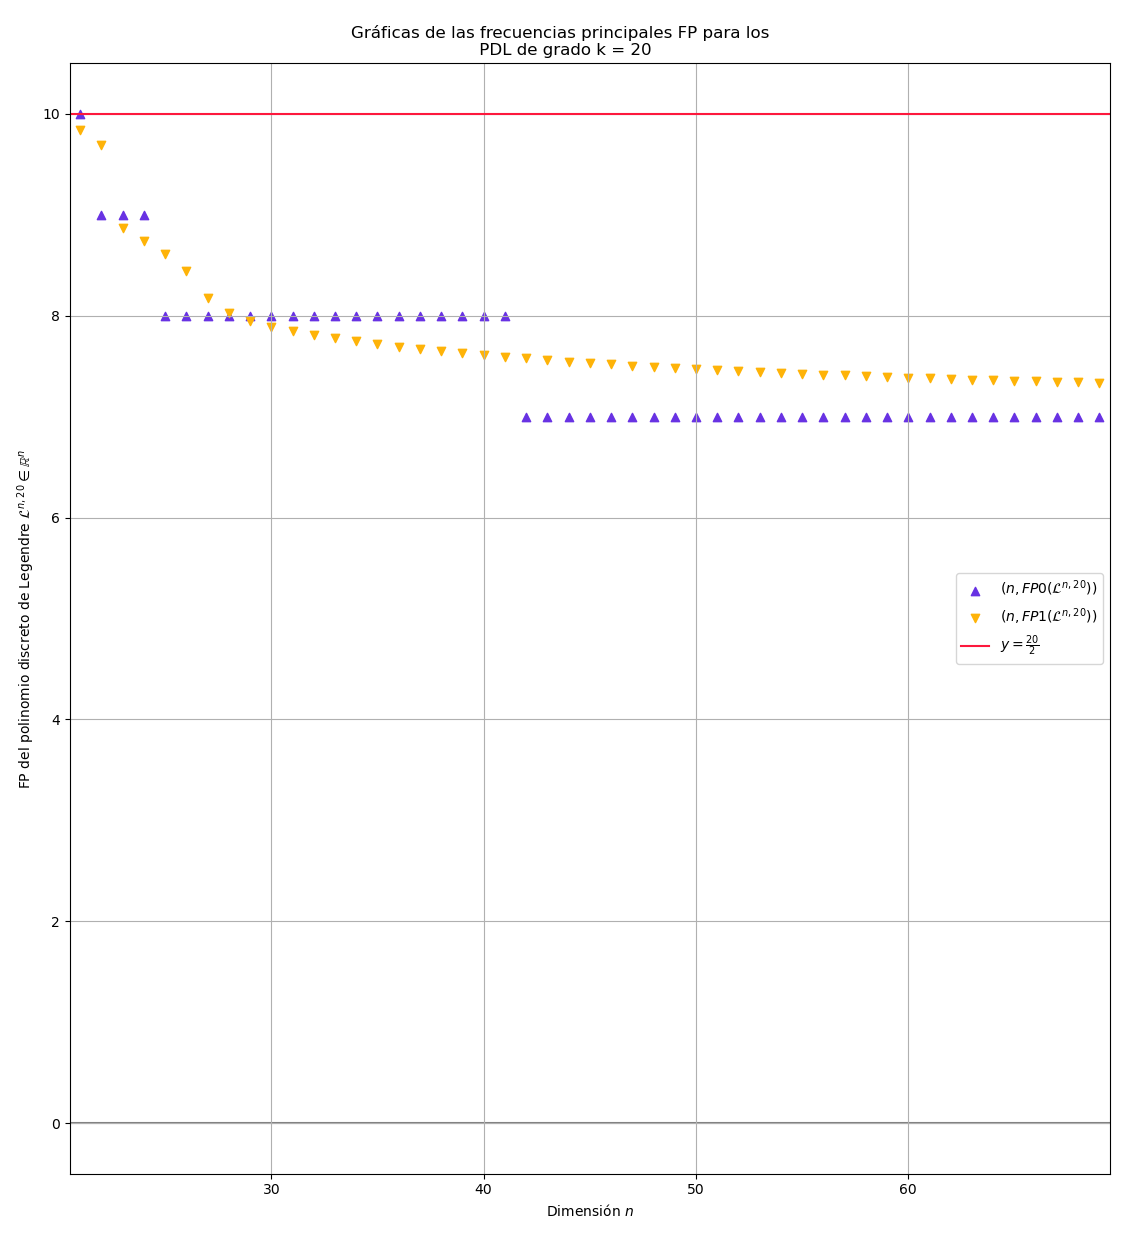
\includegraphics[scale = 0.5]{./estudios_espectrales/k_20} 
\end{figure}

\begin{figure}[H]
	\sidecaption{
	\label{fig: k 40}
	}
	\centering
	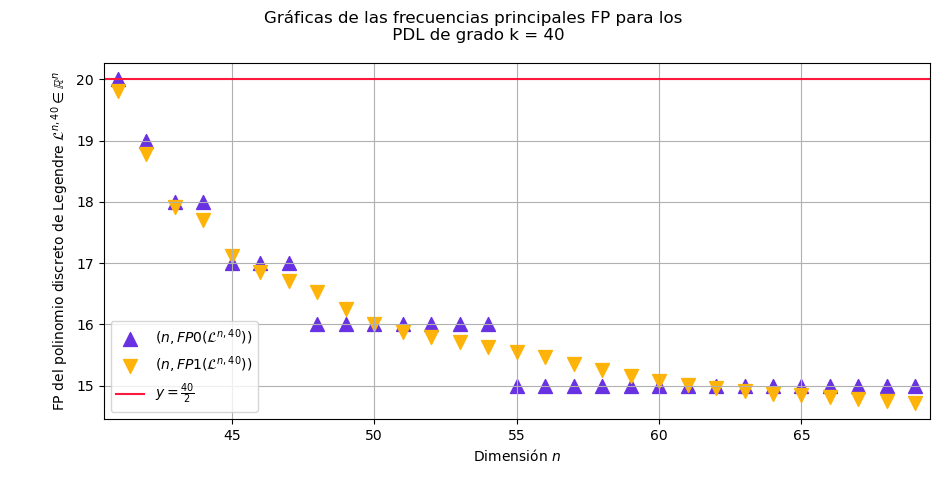
\includegraphics[scale = 0.5]{./estudios_espectrales/k_40} 
\end{figure}

\begin{figure}[H]
	\sidecaption{
	\label{fig: k 47}
	}
	\centering
	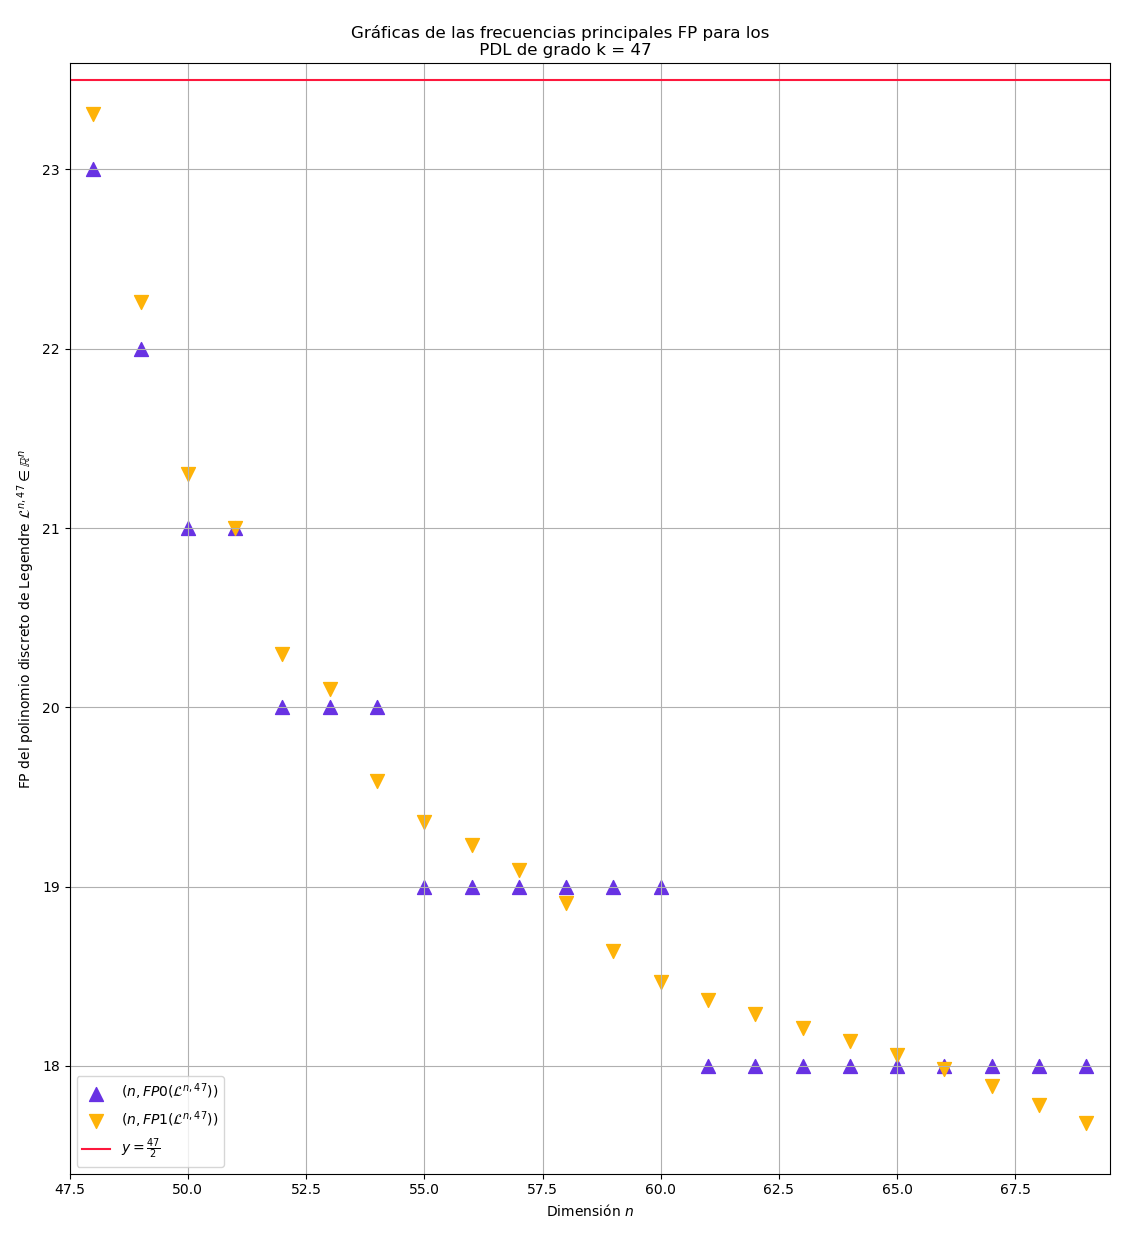
\includegraphics[scale = 0.5]{./estudios_espectrales/k_47} 
\end{figure}

\begin{figure}[H]
	\sidecaption{
	\label{fig: k 55}
	}
	\centering
	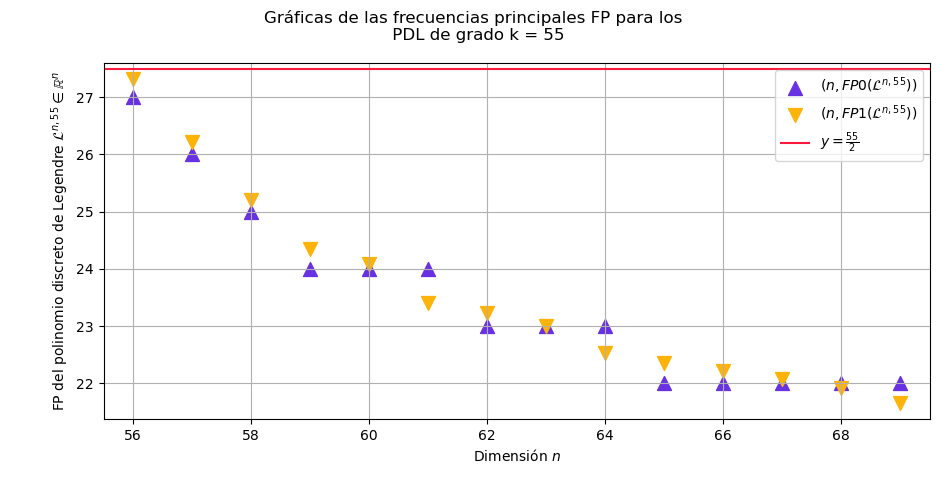
\includegraphics[scale = 0.5]{./estudios_espectrales/k_55} 
\end{figure}

Observe que, para valores de $k$ ``grandes'', parece ser que 
la frecuencia principal del PDL $\cali{L}^{n,k}$
es dependiente no sólo de $k$, sino que la dimensión $n$
también influye, y que, conforme $n$ aumenta, las
frecuencias principales disminuyen.
Lo que es constante en todas las gráficas es que 
las FP1 están siempre por debajo de
$\frac{k}{2}$.
Note además que, para valores pequeños de $k$, la diferencia
entre los valores reales de las frecuencias principales
y la estimación de $k/2$ no parece rebasar más que algunas
unidades, pero, conforme $k$ es mayor, la diferencia
es considerable (por ejemplo, en la figura \ref{fig: k 55}
puede apreciarse que algunas frecuencias principales están
a más de 5 unidades de distancia del valor estimado $55/2$
para la frecuencia principal). 

\begin{figure}[H]
	\sidecaption{
	Según la figura \eqref{fig: k 47}, la frecuencia principal
	del PDL $\cali{L}^{48, 47}$, cuyo espectro se muestra en la figura, es
	muy cercano al valor predicho $k = 44/7$. Observe que el sinusoide
	que resulta del análisis (marcado en naranja) parece aproximar
	decentemente al PDL en los extremos, pero no es capaz de 
	de modelar las oscilaciones centrales. El que no sea posible
	modelar a toda la gráfica con un sólo sinusoide se refleja
	en el hecho de que $\sigma_{n}(\cali{L}^{48,47}, FP1(\cali{L}^{48,47}))$
	(que, según la definición de frecuencia principal, es el valor
	máximo del espectro de la señal $\cali{L}^{48,47}$) es $0.77$, cuando
	el caso óptimo es que este coeficiente espectral sea
	cercano a $1$.
	\label{fig: 48 47}
	}
	\centering
	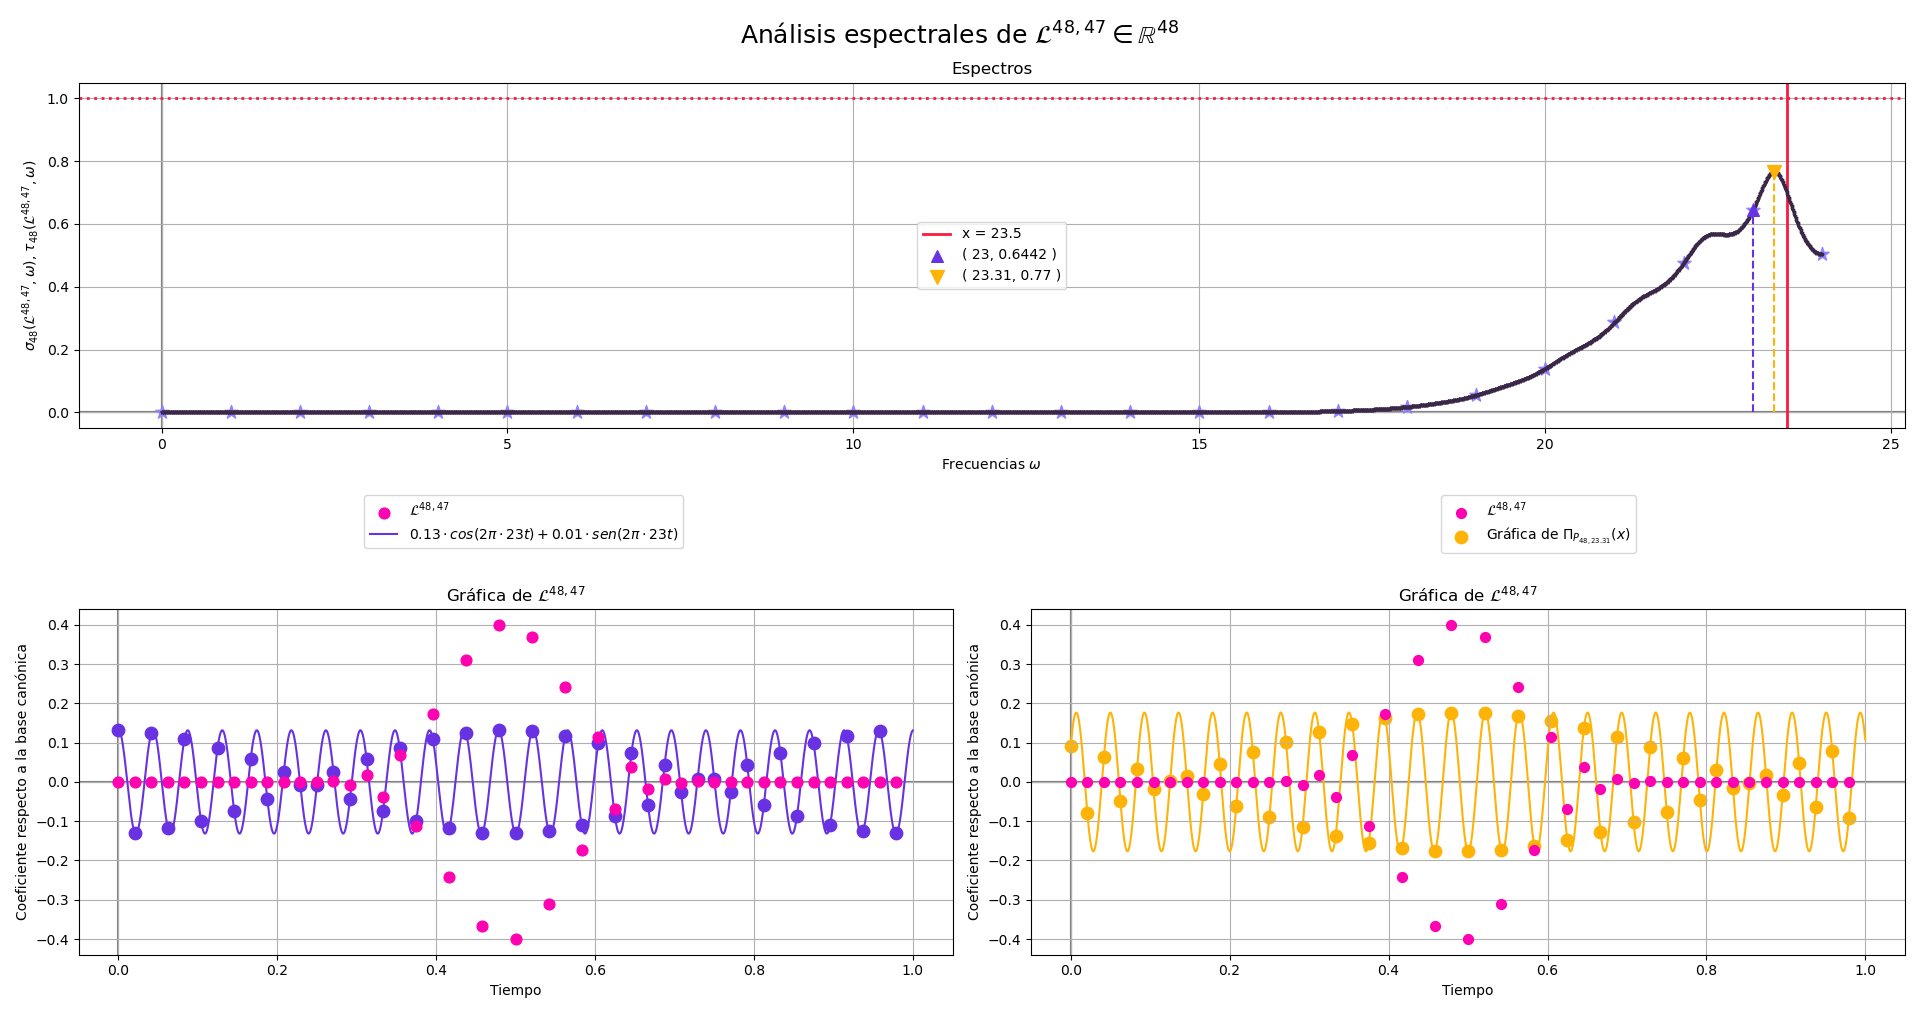
\includegraphics[angle = 90, scale = 0.4]{48_47} 
\end{figure}
\begin{figure}[H]
	\sidecaption{ Aquí, como en la figura \ref{fig: 48 47},
	se analiza el espectro de un PDL de grado $47$, pero la dimensión
	del de esta imagen es mayor (a saber, $60$) a la del PDL
	de la figura \ref{fig: 48 47}. Observe que la  
	aproximación es aún peor que la dada en \ref{fig: 48 47}, y que
	el coeficiente espectral asociado a la frecuencia principal
	es aún menos cercano a $1$.
	\label{fig: 60 47}
	}
	\centering
	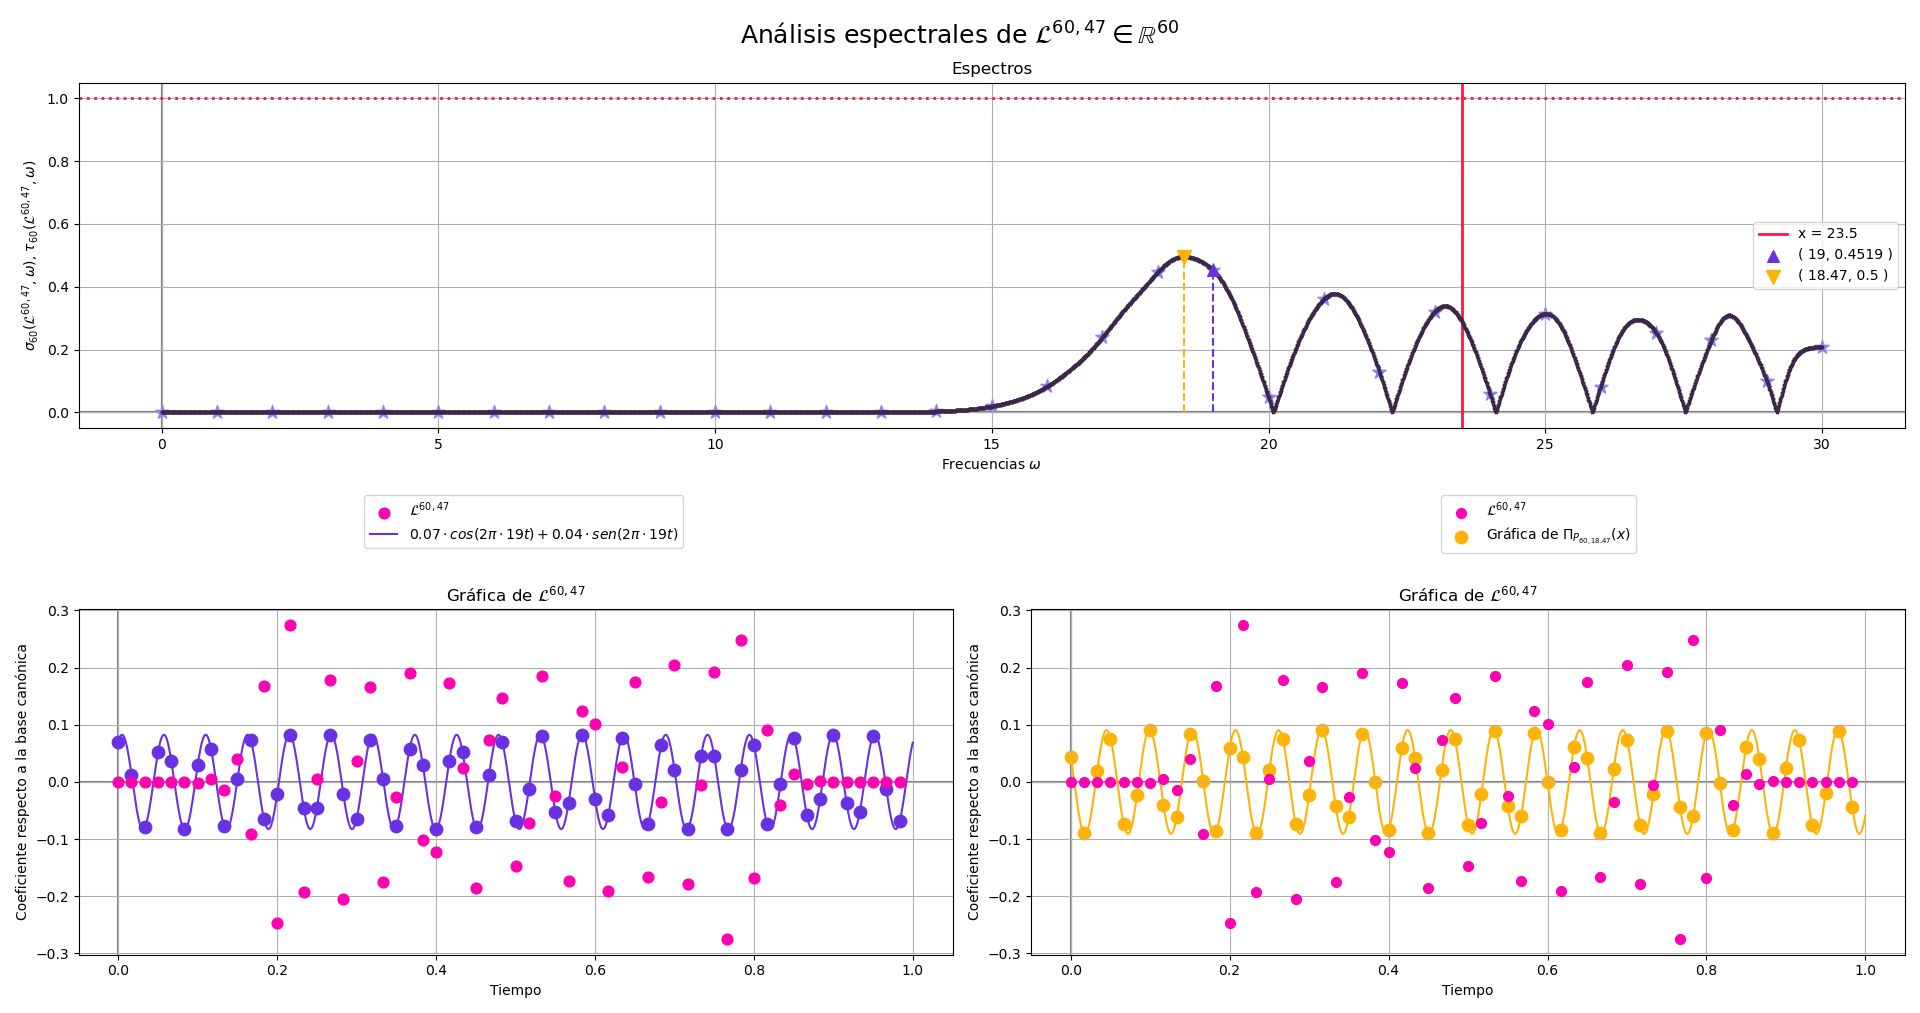
\includegraphics[angle = 90, scale = 0.4]{60_47} 
\end{figure}


Para comprobar o refutar el hecho de que, conforme $n$ 
es grande y $k$ tiende a $n-1$ (su cota superior),
los PDL de dimensión $n$ y grado $k$ no están bien
modelados con un solo sinusoide (o sea, que no parezca que les
es característica una frecuecia en particular), 
fijado un grado $k$
será de utilidad
graficar los puntos de la forma
\begin{equation}
\label{ea0: 17may}
(n, \tau_{n}(\cali{L}^{n,k}, FP0(\cali{L}^{n,k})))
\end{equation}
y
\begin{equation}
\label{ea1: 17may}
(n, \sigma_{n}(\cali{L}^{n,k}, FP1(\cali{L}^{n,k})));
\end{equation}
si ocurriése que los PDL por lo general reaccionan
principalmente a una frecuencia, se debería tener 
(según la nota 
\ref{nota: la mejor frecuencia}) que
las ordenadas de los puntos
\ref{ea0: 17may} y \ref{ea1: 17may}
son cercanas a $1$.


\begin{figure}[H]
	\sidecaption{
	\TODO{a}
	\label{fig: FP k 2}
	}
	\centering
	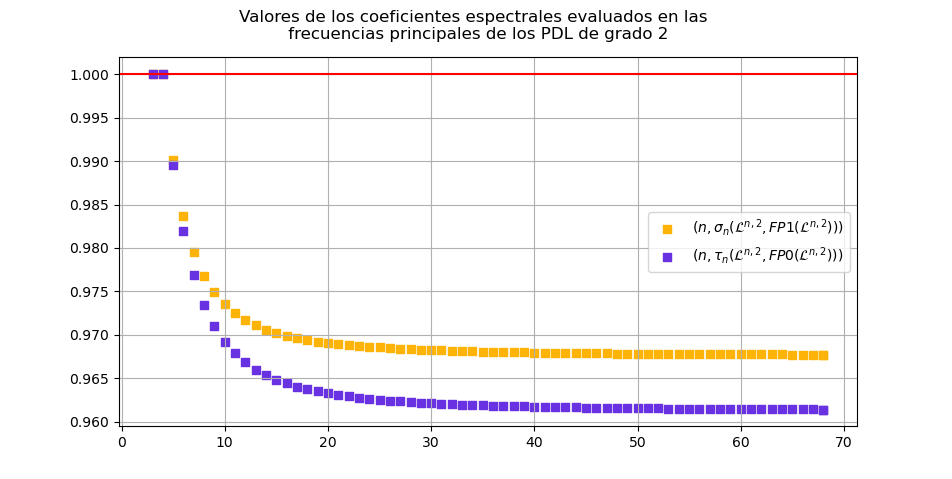
\includegraphics[scale = 0.6]{FP_k_2} 
\end{figure}	
\begin{figure}[H]
	\sidecaption{
	\TODO{a}
	\label{fig: FP k 8}
	}
	\centering
	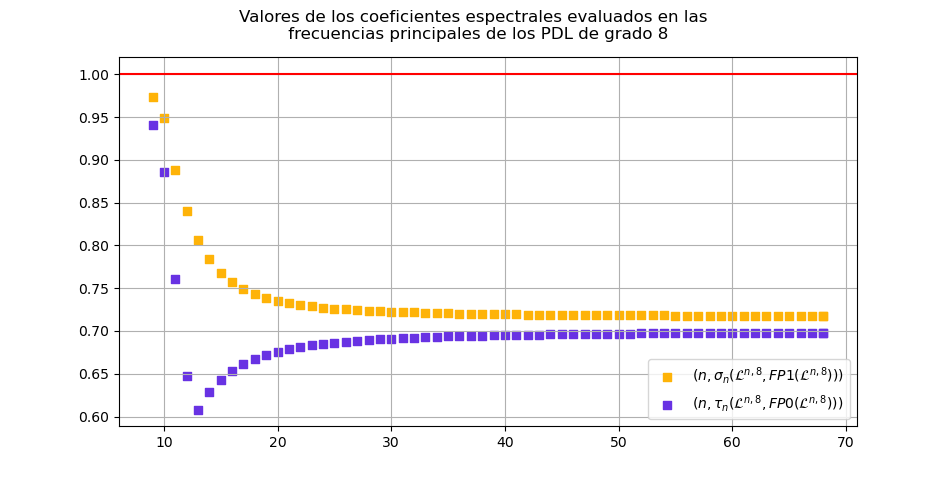
\includegraphics[scale = 0.6]{FP_k_8} 
\end{figure}	

\begin{figure}[H]
	\sidecaption{
	\TODO{a}
	\label{fig: FP k 20}
	}
	\centering
	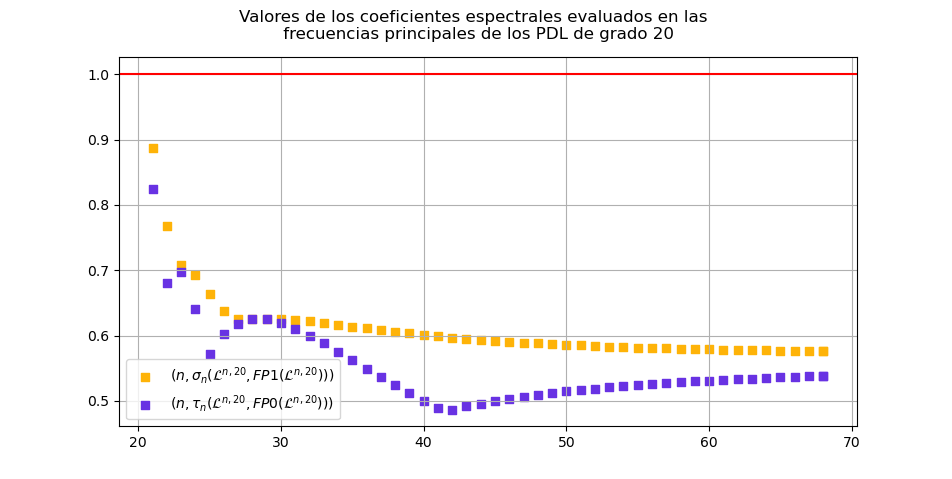
\includegraphics[scale = 0.6]{FP_k_20} 
\end{figure}	

\begin{figure}[H]
	\sidecaption{
	\TODO{a}
	\label{fig: FP k 30}
	}
	\centering
	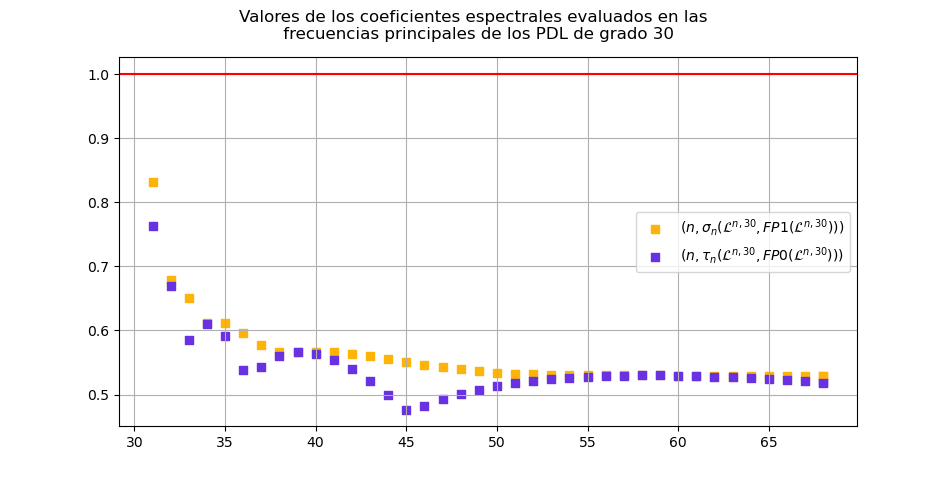
\includegraphics[scale = 0.6]{FP_k_30} 
\end{figure}	

\begin{figure}[H]
	\sidecaption{
	\TODO{a}
	\label{fig: FP k 40}
	}
	\centering
	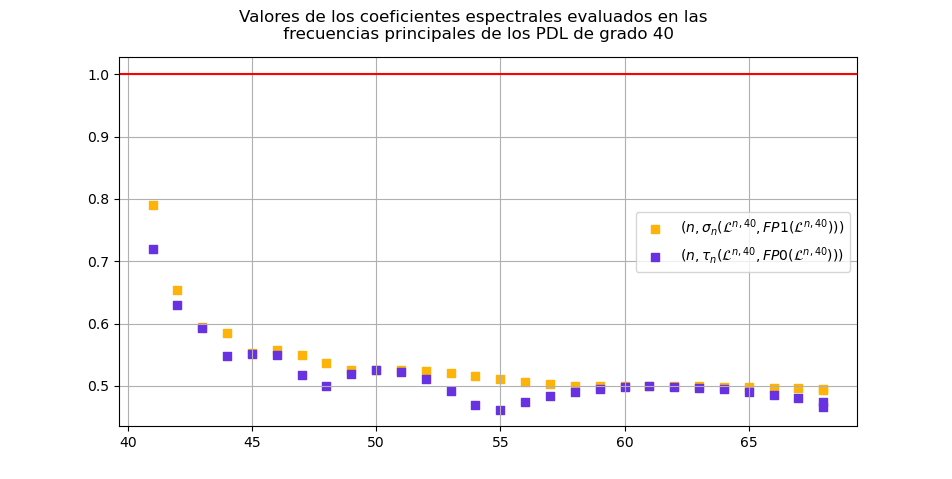
\includegraphics[scale = 0.6]{FP_k_40} 
\end{figure}	

\begin{figure}[H]
	\sidecaption{
	\TODO{a}
	\label{fig: FP k 50}
	}
	\centering
	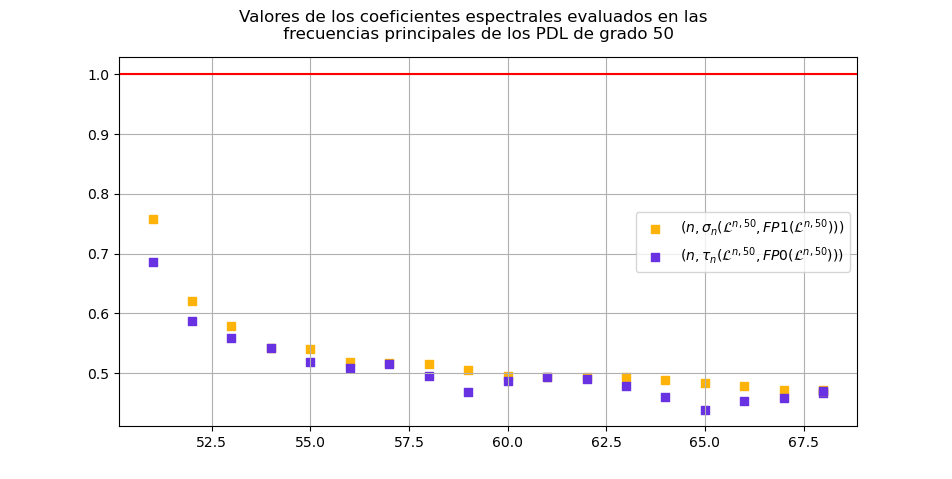
\includegraphics[scale = 0.6]{FP_k_50} 
\end{figure}	

\begin{figure}[H]
	\sidecaption{
	\TODO{a}
	\label{fig: FP k 60}
	}
	\centering
	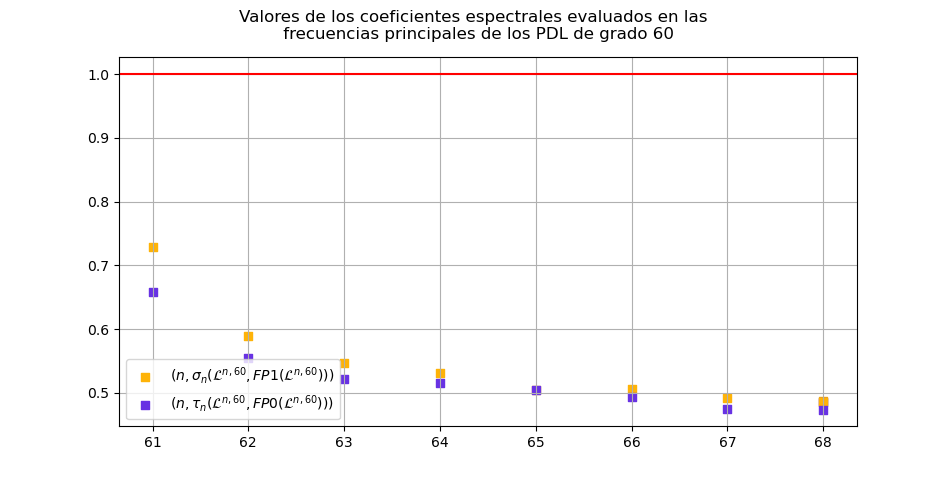
\includegraphics[scale = 0.6]{FP_k_60} 
\end{figure}	

\begin{figure}[H]
	\sidecaption{
	\TODO{a}
	\label{fig: FP k 66}
	}
	\centering
	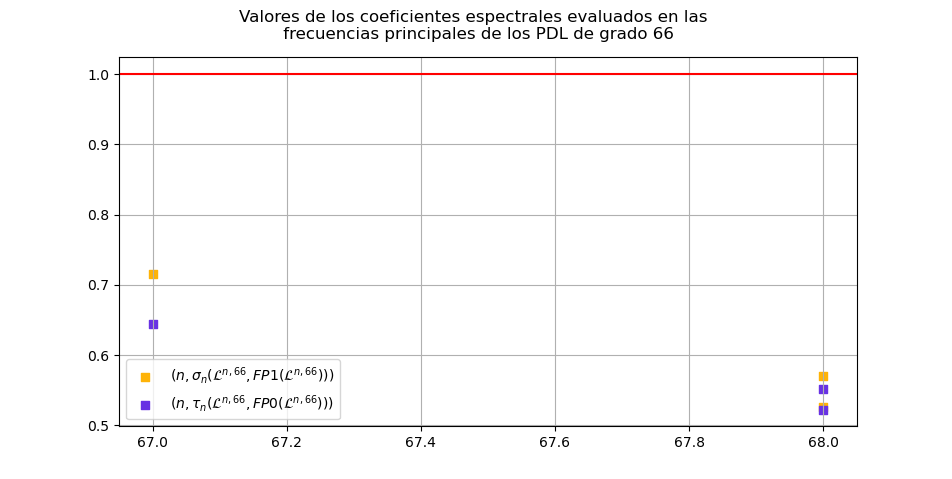
\includegraphics[scale = 0.6]{FP_k_66} 
\end{figure}	


Comprobamos que los valores de los
coeficientes espectrales de un PDL
evaluados en la frecuencia principal de este 
se alejan de $1$ (el caso ideal)
conforme $n$ aumenta y $k$ no tiene valores bajos. \\

Por otro lado, 
observe cómo los coeficientes espectrales 
$\sigma_{n}(\cali{L}^{n,k}, FP1(\cali{L}^{n,k})))$ son 
siempre más cercanos a $1$
que los 
$\tau_{n}(\cali{L}^{n,k}, FP0(\cali{L}^{n,k})))$, 
comprobando con esto que con el estudio
espectral basado en espacios monofrecuenciales
es posible encontrar una frecuencia que ajuste mejor la
gráfica del PDL que la frecuencia resultante
al hacer un análisis con la TDF.

\subsection{Lista de conclusiones}
\TODO{en construcción. Es sólo un resumen puntual
de lo anterior}
\begin{itemize}
\item Si $n$ y $k$ son ambos grandes, 
no parece ser factible aproximar la gráfica
del PDL $\cali{L}^{n,k}$ sólo con un sinusoide. Los valores
de los coeficientes espectrales $\sigma_{n}(\cali{L}^{n,k}, \omega)$
parecen estár todos muy alejados de $1$.
\item Incluso para valores grandes de $n$, los primeros
PDL de dimensión $n$ parecen tener una clara frecuencia.
\end{itemize}